\PassOptionsToPackage{unicode=true}{hyperref} % options for packages loaded elsewhere
\PassOptionsToPackage{hyphens}{url}
%
\documentclass[]{article}
\usepackage{lmodern}
\usepackage{amssymb,amsmath}
\usepackage{ifxetex,ifluatex}
\usepackage{fixltx2e} % provides \textsubscript
\ifnum 0\ifxetex 1\fi\ifluatex 1\fi=0 % if pdftex
  \usepackage[T1]{fontenc}
  \usepackage[utf8]{inputenc}
  \usepackage{textcomp} % provides euro and other symbols
\else % if luatex or xelatex
  \usepackage{unicode-math}
  \defaultfontfeatures{Ligatures=TeX,Scale=MatchLowercase}
\fi
% use upquote if available, for straight quotes in verbatim environments
\IfFileExists{upquote.sty}{\usepackage{upquote}}{}
% use microtype if available
\IfFileExists{microtype.sty}{%
\usepackage[]{microtype}
\UseMicrotypeSet[protrusion]{basicmath} % disable protrusion for tt fonts
}{}
\IfFileExists{parskip.sty}{%
\usepackage{parskip}
}{% else
\setlength{\parindent}{0pt}
\setlength{\parskip}{6pt plus 2pt minus 1pt}
}
\usepackage{hyperref}
\hypersetup{
            pdftitle={Report},
            pdfauthor={Derl Clausen, Bruno Komel, Rakeen Tanvir},
            pdfborder={0 0 0},
            breaklinks=true}
\urlstyle{same}  % don't use monospace font for urls
\usepackage[margin=1in]{geometry}
\usepackage{color}
\usepackage{fancyvrb}
\newcommand{\VerbBar}{|}
\newcommand{\VERB}{\Verb[commandchars=\\\{\}]}
\DefineVerbatimEnvironment{Highlighting}{Verbatim}{commandchars=\\\{\}}
% Add ',fontsize=\small' for more characters per line
\usepackage{framed}
\definecolor{shadecolor}{RGB}{248,248,248}
\newenvironment{Shaded}{\begin{snugshade}}{\end{snugshade}}
\newcommand{\AlertTok}[1]{\textcolor[rgb]{0.94,0.16,0.16}{#1}}
\newcommand{\AnnotationTok}[1]{\textcolor[rgb]{0.56,0.35,0.01}{\textbf{\textit{#1}}}}
\newcommand{\AttributeTok}[1]{\textcolor[rgb]{0.77,0.63,0.00}{#1}}
\newcommand{\BaseNTok}[1]{\textcolor[rgb]{0.00,0.00,0.81}{#1}}
\newcommand{\BuiltInTok}[1]{#1}
\newcommand{\CharTok}[1]{\textcolor[rgb]{0.31,0.60,0.02}{#1}}
\newcommand{\CommentTok}[1]{\textcolor[rgb]{0.56,0.35,0.01}{\textit{#1}}}
\newcommand{\CommentVarTok}[1]{\textcolor[rgb]{0.56,0.35,0.01}{\textbf{\textit{#1}}}}
\newcommand{\ConstantTok}[1]{\textcolor[rgb]{0.00,0.00,0.00}{#1}}
\newcommand{\ControlFlowTok}[1]{\textcolor[rgb]{0.13,0.29,0.53}{\textbf{#1}}}
\newcommand{\DataTypeTok}[1]{\textcolor[rgb]{0.13,0.29,0.53}{#1}}
\newcommand{\DecValTok}[1]{\textcolor[rgb]{0.00,0.00,0.81}{#1}}
\newcommand{\DocumentationTok}[1]{\textcolor[rgb]{0.56,0.35,0.01}{\textbf{\textit{#1}}}}
\newcommand{\ErrorTok}[1]{\textcolor[rgb]{0.64,0.00,0.00}{\textbf{#1}}}
\newcommand{\ExtensionTok}[1]{#1}
\newcommand{\FloatTok}[1]{\textcolor[rgb]{0.00,0.00,0.81}{#1}}
\newcommand{\FunctionTok}[1]{\textcolor[rgb]{0.00,0.00,0.00}{#1}}
\newcommand{\ImportTok}[1]{#1}
\newcommand{\InformationTok}[1]{\textcolor[rgb]{0.56,0.35,0.01}{\textbf{\textit{#1}}}}
\newcommand{\KeywordTok}[1]{\textcolor[rgb]{0.13,0.29,0.53}{\textbf{#1}}}
\newcommand{\NormalTok}[1]{#1}
\newcommand{\OperatorTok}[1]{\textcolor[rgb]{0.81,0.36,0.00}{\textbf{#1}}}
\newcommand{\OtherTok}[1]{\textcolor[rgb]{0.56,0.35,0.01}{#1}}
\newcommand{\PreprocessorTok}[1]{\textcolor[rgb]{0.56,0.35,0.01}{\textit{#1}}}
\newcommand{\RegionMarkerTok}[1]{#1}
\newcommand{\SpecialCharTok}[1]{\textcolor[rgb]{0.00,0.00,0.00}{#1}}
\newcommand{\SpecialStringTok}[1]{\textcolor[rgb]{0.31,0.60,0.02}{#1}}
\newcommand{\StringTok}[1]{\textcolor[rgb]{0.31,0.60,0.02}{#1}}
\newcommand{\VariableTok}[1]{\textcolor[rgb]{0.00,0.00,0.00}{#1}}
\newcommand{\VerbatimStringTok}[1]{\textcolor[rgb]{0.31,0.60,0.02}{#1}}
\newcommand{\WarningTok}[1]{\textcolor[rgb]{0.56,0.35,0.01}{\textbf{\textit{#1}}}}
\usepackage{graphicx,grffile}
\makeatletter
\def\maxwidth{\ifdim\Gin@nat@width>\linewidth\linewidth\else\Gin@nat@width\fi}
\def\maxheight{\ifdim\Gin@nat@height>\textheight\textheight\else\Gin@nat@height\fi}
\makeatother
% Scale images if necessary, so that they will not overflow the page
% margins by default, and it is still possible to overwrite the defaults
% using explicit options in \includegraphics[width, height, ...]{}
\setkeys{Gin}{width=\maxwidth,height=\maxheight,keepaspectratio}
\setlength{\emergencystretch}{3em}  % prevent overfull lines
\providecommand{\tightlist}{%
  \setlength{\itemsep}{0pt}\setlength{\parskip}{0pt}}
\setcounter{secnumdepth}{0}
% Redefines (sub)paragraphs to behave more like sections
\ifx\paragraph\undefined\else
\let\oldparagraph\paragraph
\renewcommand{\paragraph}[1]{\oldparagraph{#1}\mbox{}}
\fi
\ifx\subparagraph\undefined\else
\let\oldsubparagraph\subparagraph
\renewcommand{\subparagraph}[1]{\oldsubparagraph{#1}\mbox{}}
\fi

% set default figure placement to htbp
\makeatletter
\def\fps@figure{htbp}
\makeatother


\title{Report}
\author{Derl Clausen, Bruno Komel, Rakeen Tanvir}
\date{5/11/2020}

\begin{document}
\maketitle

\#Outline Exploratory Data Analysis The Impact of ``Rare'' Events Linear
and Logistic Regression Fourier Analysis Random Walk Normal Distribution
Fractal Analysis Cauchy Distribution Bootstrap Partial Variance
Divergent Integration Stable Distribution KS Test / Chi-Squared Test
(Chi-square Test on Varying Time Scales) / Complexities of Goodness of
Fit Test The Impact of Political Regimes - Hypothesis Testing With
Permutation Test Hypothesis Testing: Contingency table with chi-square
test

\#Exploratory Data Analysis The first differences of DJI Open price
values present an interesting challenge. The histogram resembles a
symmetric distribution with a sharp peak around the mean, heavy tails,
and a left skew. The normal distribution does not seem to be a good fit
at first glance, but a heavy-tailed distribution could help us model our
data

\begin{Shaded}
\begin{Highlighting}[]
\CommentTok{#Import libraries}
\KeywordTok{library}\NormalTok{(}\StringTok{'pracma'}\NormalTok{)}
\KeywordTok{library}\NormalTok{(}\StringTok{'fitdistrplus'}\NormalTok{)}
\end{Highlighting}
\end{Shaded}

\begin{verbatim}
## Loading required package: MASS
\end{verbatim}

\begin{verbatim}
## Warning: package 'MASS' was built under R version 3.6.2
\end{verbatim}

\begin{verbatim}
## Loading required package: survival
\end{verbatim}

\begin{verbatim}
## Loading required package: npsurv
\end{verbatim}

\begin{verbatim}
## Loading required package: lsei
\end{verbatim}

\begin{Shaded}
\begin{Highlighting}[]
\KeywordTok{library}\NormalTok{(}\StringTok{'MASS'}\NormalTok{)}
\KeywordTok{library}\NormalTok{(}\StringTok{'ggplot2'}\NormalTok{)}
\KeywordTok{library}\NormalTok{(}\StringTok{'gganimate'}\NormalTok{)}
\KeywordTok{library}\NormalTok{(}\StringTok{'gifski'}\NormalTok{)}
\KeywordTok{library}\NormalTok{(}\StringTok{'fractaldim'}\NormalTok{)}
\end{Highlighting}
\end{Shaded}

\begin{verbatim}
## Loading required package: abind
\end{verbatim}

\begin{Shaded}
\begin{Highlighting}[]
\KeywordTok{library}\NormalTok{(}\StringTok{'fBasics'}\NormalTok{)}
\end{Highlighting}
\end{Shaded}

\begin{verbatim}
## Loading required package: timeDate
\end{verbatim}

\begin{verbatim}
## Loading required package: timeSeries
\end{verbatim}

\begin{verbatim}
## 
## Attaching package: 'fBasics'
\end{verbatim}

\begin{verbatim}
## The following objects are masked from 'package:pracma':
## 
##     akimaInterp, inv, kron, pascal
\end{verbatim}

\begin{Shaded}
\begin{Highlighting}[]
\KeywordTok{library}\NormalTok{(}\StringTok{'stabledist'}\NormalTok{)}
\KeywordTok{library}\NormalTok{(}\StringTok{'car'}\NormalTok{)}
\end{Highlighting}
\end{Shaded}

\begin{verbatim}
## Loading required package: carData
\end{verbatim}

\begin{verbatim}
## 
## Attaching package: 'car'
\end{verbatim}

\begin{verbatim}
## The following object is masked from 'package:fBasics':
## 
##     densityPlot
\end{verbatim}

\begin{verbatim}
## The following object is masked from 'package:pracma':
## 
##     logit
\end{verbatim}

\begin{Shaded}
\begin{Highlighting}[]
\KeywordTok{source}\NormalTok{(}\StringTok{'prj_DataPreparation.R'}\NormalTok{)}
\KeywordTok{source}\NormalTok{(}\StringTok{'prj_Functions.R'}\NormalTok{)}


\CommentTok{#This is a graphical representation of the Dow Jones Index from 1985 to 2020}
\KeywordTok{plot}\NormalTok{(DJI}\OperatorTok{$}\NormalTok{Open, }\DataTypeTok{type =} \StringTok{"l"}\NormalTok{, }\DataTypeTok{xlab =} \StringTok{"Time"}\NormalTok{, }
     \DataTypeTok{ylab =} \StringTok{"Random Daily Opens"}\NormalTok{, }\DataTypeTok{main =} \StringTok{"Random Walk Model"}\NormalTok{,}
     \DataTypeTok{ylim =} \KeywordTok{c}\NormalTok{(}\OperatorTok{-}\DecValTok{10000}\NormalTok{,}\DecValTok{50000}\NormalTok{))}
\end{Highlighting}
\end{Shaded}

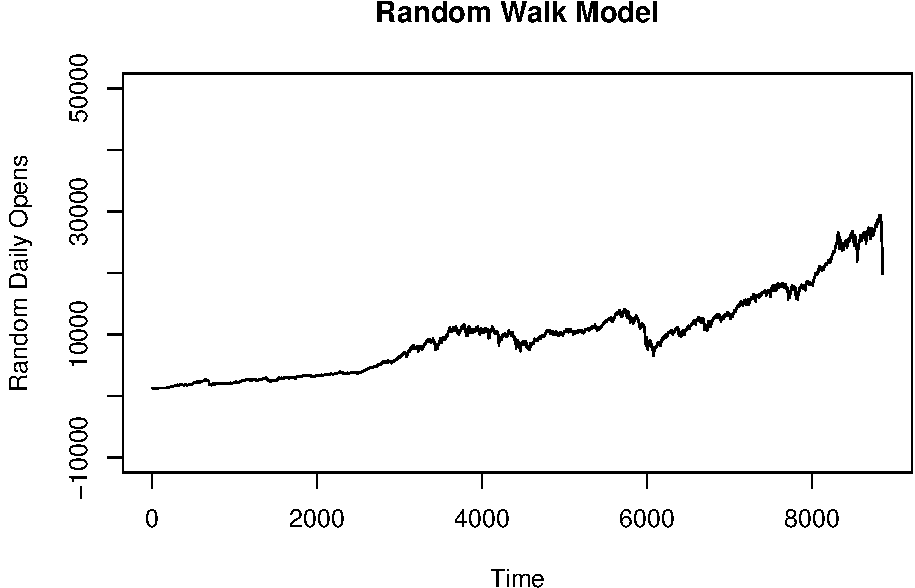
\includegraphics{Report_files/figure-latex/unnamed-chunk-1-1.pdf}

\begin{Shaded}
\begin{Highlighting}[]
\CommentTok{#Get the first difference of the time series data}
\NormalTok{diffs <-}\StringTok{ }\KeywordTok{diff}\NormalTok{(DJI}\OperatorTok{$}\NormalTok{Open)}
\end{Highlighting}
\end{Shaded}

\#The Impact of ``Rare'' Events Let's begin by taking a look at
presumably rare events, and how they're represented in our data. Let's
consider each of the days where was a statistically significant price
change assuming these price changes followed a normal distribution.

\begin{Shaded}
\begin{Highlighting}[]
\NormalTok{mu <-}\StringTok{ }\KeywordTok{mean}\NormalTok{(diffs); mu}
\end{Highlighting}
\end{Shaded}

\begin{verbatim}
## [1] 2.142422
\end{verbatim}

\begin{Shaded}
\begin{Highlighting}[]
\NormalTok{sigma <-}\StringTok{ }\KeywordTok{sd}\NormalTok{(diffs); sigma}
\end{Highlighting}
\end{Shaded}

\begin{verbatim}
## [1] 117.3051
\end{verbatim}

\begin{Shaded}
\begin{Highlighting}[]
\NormalTok{N <-}\StringTok{ }\KeywordTok{length}\NormalTok{(diffs)}
\NormalTok{SDs <-}\StringTok{ }\KeywordTok{numeric}\NormalTok{(N)}
\ControlFlowTok{for}\NormalTok{ (i }\ControlFlowTok{in} \DecValTok{1}\OperatorTok{:}\NormalTok{N)\{}
\NormalTok{  SDs[i] <-}\StringTok{ }\NormalTok{(diffs[i]}\OperatorTok{-}\NormalTok{mu)}\OperatorTok{/}\NormalTok{sigma}
\NormalTok{\}}
\KeywordTok{head}\NormalTok{(SDs);}\KeywordTok{head}\NormalTok{(diffs)}
\end{Highlighting}
\end{Shaded}

\begin{verbatim}
## [1]  0.14924841 -0.13871881 -0.07197018 -0.05969396  0.16911181 -0.09643625
\end{verbatim}

\begin{verbatim}
## [1]  19.650024 -14.130005  -6.300049  -4.859985  21.980103  -9.170044
\end{verbatim}

\begin{Shaded}
\begin{Highlighting}[]
\KeywordTok{length}\NormalTok{(SDs)}
\end{Highlighting}
\end{Shaded}

\begin{verbatim}
## [1] 8857
\end{verbatim}

\begin{Shaded}
\begin{Highlighting}[]
\NormalTok{SDs.data <-}\StringTok{ }\KeywordTok{c}\NormalTok{(}\DecValTok{0}\NormalTok{,SDs[}\DecValTok{1}\OperatorTok{:}\KeywordTok{length}\NormalTok{(SDs)]); }\KeywordTok{head}\NormalTok{(SDs.data) }
\end{Highlighting}
\end{Shaded}

\begin{verbatim}
## [1]  0.00000000  0.14924841 -0.13871881 -0.07197018 -0.05969396  0.16911181
\end{verbatim}

\begin{Shaded}
\begin{Highlighting}[]
\NormalTok{DJI <-}\StringTok{ }\KeywordTok{data.frame}\NormalTok{(DJI,SDs.data)}
\NormalTok{idx <-}\StringTok{ }\KeywordTok{which}\NormalTok{(}\KeywordTok{abs}\NormalTok{(SDs.data) }\OperatorTok{>}\StringTok{ }\DecValTok{5}\NormalTok{); }\KeywordTok{head}\NormalTok{(idx)}
\end{Highlighting}
\end{Shaded}

\begin{verbatim}
## [1] 3846 4200 5971 5979 5981 5983
\end{verbatim}

\begin{Shaded}
\begin{Highlighting}[]
\NormalTok{unusual <-}\StringTok{ }\NormalTok{DJI[idx,]; }\KeywordTok{head}\NormalTok{(unusual) }
\end{Highlighting}
\end{Shaded}

\begin{verbatim}
##            Date     Open     High      Low    Close Adj.Close    Volume Regime
## 3846 2000-04-17 10303.29 10583.75 10232.55 10582.51  10582.51 247520000     BC
## 4200 2001-09-18  8922.70  9022.06  8861.05  8903.40   8903.40 372230000    GWB
## 5971 2008-09-30 10371.58 10868.90 10371.42 10850.66  10850.66 319770000    GWB
## 5979 2008-10-10  8568.67  8901.28  7882.51  8451.19   8451.19 674920000    GWB
## 5981 2008-10-14  9388.97  9794.37  9085.43  9310.99   9310.99 412740000    GWB
## 5983 2008-10-16  8577.04  9013.27  8197.67  8979.26   8979.26 422450000    GWB
##      Republican Recession     diffs  SDs.data
## 3846      FALSE     FALSE -619.5596 -5.299871
## 4200       TRUE      TRUE -657.6201 -5.624329
## 5971       TRUE      TRUE -768.0400 -6.565634
## 5979       TRUE      TRUE -693.0205 -5.926109
## 5981       TRUE      TRUE  926.5498  7.880367
## 5983       TRUE      TRUE -724.8701 -6.197620
\end{verbatim}

As we can see, there are 32 days in which the price flux for the Dow
Jones was larger than 5 standard deviations away from the mean. To show
just how bad of a fit the assume of normal distribution is for our data
consider the p-values for each of these events.

\begin{Shaded}
\begin{Highlighting}[]
\NormalTok{N <-}\StringTok{ }\KeywordTok{nrow}\NormalTok{(unusual)}
\NormalTok{pvals <-}\StringTok{ }\KeywordTok{numeric}\NormalTok{(N)}
\ControlFlowTok{for}\NormalTok{ (i }\ControlFlowTok{in} \DecValTok{1}\OperatorTok{:}\NormalTok{(N)) \{}
\NormalTok{ pvals[i] <-}\StringTok{ }\KeywordTok{pnorm}\NormalTok{(}\KeywordTok{abs}\NormalTok{(unusual}\OperatorTok{$}\NormalTok{SDs.data[i]}\OperatorTok{*}\NormalTok{sigma), }\DataTypeTok{mean =}\NormalTok{ mu, }\DataTypeTok{sd =}\NormalTok{ sigma, }\DataTypeTok{lower.tail =} \OtherTok{FALSE}\NormalTok{)}
\NormalTok{\}}
\KeywordTok{head}\NormalTok{(pvals)}
\end{Highlighting}
\end{Shaded}

\begin{verbatim}
## [1] 6.402775e-08 1.034892e-08 2.927955e-11 1.733056e-09 1.888683e-15
## [6] 3.218177e-10
\end{verbatim}

\begin{Shaded}
\begin{Highlighting}[]
\NormalTok{rare <-}\StringTok{ }\KeywordTok{max}\NormalTok{(pvals);rare }\CommentTok{#2.303366e-07, which is pretty much 0. }
\end{Highlighting}
\end{Shaded}

\begin{verbatim}
## [1] 2.306794e-07
\end{verbatim}

\begin{Shaded}
\begin{Highlighting}[]
\NormalTok{(}\DecValTok{1}\OperatorTok{/}\NormalTok{rare)}\OperatorTok{/}\DecValTok{365}
\end{Highlighting}
\end{Shaded}

\begin{verbatim}
## [1] 11876.77
\end{verbatim}

If we interpret the p-value as the probability of an event taking place,
and our events are measured in days, then a given p-value tells us the
probability of seeing that extreme of an event on any given days (i.e.~a
p-value of 0.05 would correspond to an event that we'd ``expect'' to see
once every 20 days, since it has a 1/20 chance of arising).In other
words, if the DJI first differences followed a normal distribution,we
would expect to see the least rare of these rare events once in
11,894.45 years, but from the data it is clear that these events are far
more common than that.

This raises two questions, does the stock market have properties of
random walk? And, if so, what is the underlying distribution of the step
size of the random walk?

\#Fourier Analysis Before analyzing our data for properties of a random
walk and infinite variance, we first need to run a Fourier Analysis to
ensure there is no cyclic patterns in our data:

\begin{Shaded}
\begin{Highlighting}[]
\CommentTok{#We will begin analysing the Open Stock Price Data before shifting into it's first difference (or price change).}
\CommentTok{#Using our RunFourier() function defined in Main.R, we check that we can fully reconstruct our data from the basis vectors:}
\KeywordTok{RunFourier}\NormalTok{(}\KeywordTok{length}\NormalTok{(DJI}\OperatorTok{$}\NormalTok{Open)}\OperatorTok{/}\DecValTok{2}\NormalTok{, DJI}\OperatorTok{$}\NormalTok{Open, }\OtherTok{FALSE}\NormalTok{) }\CommentTok{#Perfect Reconstruction }
\end{Highlighting}
\end{Shaded}

\includegraphics{Report_files/figure-latex/unnamed-chunk-4-1.pdf}

\begin{Shaded}
\begin{Highlighting}[]
\KeywordTok{RunFourier}\NormalTok{(}\DecValTok{10}\NormalTok{, DJI}\OperatorTok{$}\NormalTok{Open, }\OtherTok{FALSE}\NormalTok{) }\CommentTok{#Using only 10 basis vectors}
\end{Highlighting}
\end{Shaded}

\includegraphics{Report_files/figure-latex/unnamed-chunk-4-2.pdf}

\begin{Shaded}
\begin{Highlighting}[]
\CommentTok{#We capture the general shifts of the market using very few basis vectors in our analysis.}
\CommentTok{#As you can see, there is no discernable cyclical pattern.}

\CommentTok{#Next run Fourier Analysis on the stock price change over trading days. Again, we look for a perfect reconstruction:}
\KeywordTok{RunFourier}\NormalTok{(}\KeywordTok{length}\NormalTok{(diffs) }\OperatorTok{/}\DecValTok{2}\NormalTok{, diffs, }\OtherTok{TRUE}\NormalTok{) }\CommentTok{#Excellent}
\end{Highlighting}
\end{Shaded}

\includegraphics{Report_files/figure-latex/unnamed-chunk-4-3.pdf}

\begin{Shaded}
\begin{Highlighting}[]
\CommentTok{#Next we test it using 1000 basis vectors}
\KeywordTok{RunFourier}\NormalTok{(}\DecValTok{1000}\NormalTok{, diffs, }\OtherTok{TRUE}\NormalTok{) }\CommentTok{#No discernable pattern}
\end{Highlighting}
\end{Shaded}

\includegraphics{Report_files/figure-latex/unnamed-chunk-4-4.pdf}

\begin{Shaded}
\begin{Highlighting}[]
\CommentTok{#Check 10 basis vectors, again to see if there is any kind of pattern:}
\KeywordTok{RunFourier}\NormalTok{(}\DecValTok{10}\NormalTok{, diffs, }\OtherTok{TRUE}\NormalTok{)}
\end{Highlighting}
\end{Shaded}

\includegraphics{Report_files/figure-latex/unnamed-chunk-4-5.pdf}

\begin{Shaded}
\begin{Highlighting}[]
\CommentTok{#Using a small number of basis vectors yields no new information. Although we can}
\CommentTok{#perfectly reconstruct the data, the more basis vectors added to our analysis mostly just}
\CommentTok{#pick up on noise. Again, there is no noticeable trend or cycle which indicate we can}
\CommentTok{#proceed to examine randoms walks.}
\end{Highlighting}
\end{Shaded}

\#Random Walk with Infinite Variance Demonstration (Introduction) As we
will show, a simple plot of our data resembles a random walk. But if it
is a random walk, what kind of random walk is it? This is a good moment
to introduce Benoit Mandelbrot's research from 1963. While analyzing
stock prices, he associated two to three different probablility laws
that describe the length of the step of a random walk: Gaussian, Levy
Flight and the less popular Cauchy Flight. These probability laws are
associated with the underlying distribution of the price changes over
time. For instance, if a set of stock prices are a Gaussian random walk,
their price change over time (first difference) follows a normal
distribution, Levy flight follows a (Levy-Pareto) stable distribution,
and Cauchy Flight follows a Cauchy distribution. Using our stock price
data, we demonstrate the relationship between random walks, and the
distribution of their first difference:

\begin{Shaded}
\begin{Highlighting}[]
\CommentTok{## We begin our test by assuming our data is a Gaussian random walk model created using a (0,1,0) Arima Time Series with a Drift.}

\CommentTok{#Because we are assuming our data is a Gaussian random walk, we assume our data has finite mean and variance. Therefore we can calculate the mean and standard deviation of the first difference to model a random walk:}
\NormalTok{mu.chg.open <-}\StringTok{ }\KeywordTok{mean}\NormalTok{(diffs); mu.chg.open }\CommentTok{# 2.142422 }
\end{Highlighting}
\end{Shaded}

\begin{verbatim}
## [1] 2.142422
\end{verbatim}

\begin{Shaded}
\begin{Highlighting}[]
\NormalTok{sd.diff <-}\StringTok{ }\KeywordTok{sqrt}\NormalTok{(}\KeywordTok{mean}\NormalTok{(diffs}\OperatorTok{^}\DecValTok{2}\NormalTok{) }\OperatorTok{-}\StringTok{ }\KeywordTok{mean}\NormalTok{(diffs)); sd.diff }\CommentTok{#117.3089}
\end{Highlighting}
\end{Shaded}

\begin{verbatim}
## [1] 117.3089
\end{verbatim}

\begin{Shaded}
\begin{Highlighting}[]
\CommentTok{#Next, we plot our original data (black), with our random walk model (red):}
\KeywordTok{plot}\NormalTok{(DJI}\OperatorTok{$}\NormalTok{Open, }\DataTypeTok{type =} \StringTok{"l"}\NormalTok{, }\DataTypeTok{xlab =} \StringTok{"Time"}\NormalTok{, }
     \DataTypeTok{ylab =} \StringTok{"Random Daily Opens"}\NormalTok{, }\DataTypeTok{main =} \StringTok{"DJI Stock Price Data with 1 Simulation of Random Walk Model"}\NormalTok{,}
     \DataTypeTok{ylim =} \KeywordTok{c}\NormalTok{(}\OperatorTok{-}\DecValTok{10000}\NormalTok{,}\DecValTok{50000}\NormalTok{), }\DataTypeTok{lwd =}\DecValTok{2}\NormalTok{)}
\NormalTok{rw.drift <-}\StringTok{ }\KeywordTok{arima.sim}\NormalTok{(}\DataTypeTok{model =} \KeywordTok{list}\NormalTok{(}\DataTypeTok{order =} \KeywordTok{c}\NormalTok{(}\DecValTok{0}\NormalTok{,}\DecValTok{1}\NormalTok{,}\DecValTok{0}\NormalTok{)), }
                        \KeywordTok{length}\NormalTok{(DJI}\OperatorTok{$}\NormalTok{Open), }\DataTypeTok{mean =}\NormalTok{ mu.chg.open,}
                        \DataTypeTok{sd =}\NormalTok{ sd.diff)}
\KeywordTok{lines}\NormalTok{(rw.drift, }\DataTypeTok{col =} \StringTok{"red"}\NormalTok{)}
\end{Highlighting}
\end{Shaded}

\includegraphics{Report_files/figure-latex/unnamed-chunk-5-1.pdf}

To show the full impact of the stock market as a random walk, we run a
simulation of our model 100 times:

\begin{Shaded}
\begin{Highlighting}[]
\CommentTok{#Plot our original data}
\KeywordTok{plot}\NormalTok{(DJI}\OperatorTok{$}\NormalTok{Open, }\DataTypeTok{type =} \StringTok{"l"}\NormalTok{, }\DataTypeTok{xlab =} \StringTok{"Time"}\NormalTok{, }
     \DataTypeTok{ylab =} \StringTok{"Random Daily Opens"}\NormalTok{, }\DataTypeTok{main =} \StringTok{"100 Simulations of Random Walk Model"}\NormalTok{,}
     \DataTypeTok{ylim =} \KeywordTok{c}\NormalTok{(}\OperatorTok{-}\DecValTok{10000}\NormalTok{,}\DecValTok{50000}\NormalTok{), }\DataTypeTok{lwd =}\DecValTok{2}\NormalTok{)}

\CommentTok{#Plot of our 100 simulations:}
\ControlFlowTok{for}\NormalTok{ (i }\ControlFlowTok{in} \DecValTok{1}\OperatorTok{:}\DecValTok{100}\NormalTok{) \{}
\NormalTok{  rw.drift <-}\StringTok{ }\KeywordTok{arima.sim}\NormalTok{(}\DataTypeTok{model =} \KeywordTok{list}\NormalTok{(}\DataTypeTok{order =} \KeywordTok{c}\NormalTok{(}\DecValTok{0}\NormalTok{,}\DecValTok{1}\NormalTok{,}\DecValTok{0}\NormalTok{)), }
                        \KeywordTok{length}\NormalTok{(DJI}\OperatorTok{$}\NormalTok{Open), }\DataTypeTok{mean =}\NormalTok{ mu.chg.open,}
                        \DataTypeTok{sd =}\NormalTok{ sd.diff)}
  \KeywordTok{lines}\NormalTok{(rw.drift, }\DataTypeTok{col =} \KeywordTok{rgb}\NormalTok{(}\KeywordTok{runif}\NormalTok{(}\DecValTok{1}\NormalTok{,}\DecValTok{0}\NormalTok{,}\DecValTok{1}\NormalTok{),}\KeywordTok{runif}\NormalTok{(}\DecValTok{1}\NormalTok{,}\DecValTok{0}\NormalTok{,}\DecValTok{1}\NormalTok{),}\KeywordTok{runif}\NormalTok{(}\DecValTok{1}\NormalTok{,}\DecValTok{0}\NormalTok{,}\DecValTok{1}\NormalTok{)))}
\NormalTok{\}}
\end{Highlighting}
\end{Shaded}

\includegraphics{Report_files/figure-latex/unnamed-chunk-6-1.pdf}

\#Normal Distribution Under a gaussian random walk assumption with
finite mean and variance, our model takes on a significant range of
values across the 100 simulations. We even experience some fairly
significant volatility in certain outlier simulations that could
potentially represent a sharp drop in stock prices, perhaps, from a
recession. Therefore, it is tempting to stop here and assume our data is
a Gaussian random walk. However, our model is based on finite variance
and mean calculated from a sample rather than the population. Therefore,
to fully understand what probability laws our data is following, we need
to exmaine the first difference histograms of our data and our model.
Then, we will compare the distributions.

\begin{Shaded}
\begin{Highlighting}[]
\CommentTok{#Plot the distribution of our model and overlay a normal density curve:}
\KeywordTok{hist}\NormalTok{(}\KeywordTok{diff}\NormalTok{(rw.drift), }\DataTypeTok{breaks =} \StringTok{"FD"}\NormalTok{, }\DataTypeTok{freq =} \OtherTok{FALSE}\NormalTok{, }\DataTypeTok{main =} \StringTok{"Histogram of Random Walk Model First Difference"}\NormalTok{, }\DataTypeTok{xlab =} \StringTok{"Price Change"}\NormalTok{)}
\KeywordTok{curve}\NormalTok{(}\KeywordTok{dnorm}\NormalTok{(x, }\KeywordTok{mean}\NormalTok{(diffs), }\KeywordTok{sd}\NormalTok{(diffs)), }\DataTypeTok{add =} \OtherTok{TRUE}\NormalTok{, }\DataTypeTok{lwd =} \DecValTok{2}\NormalTok{, }\DataTypeTok{col =} \StringTok{"red"}\NormalTok{)}
\end{Highlighting}
\end{Shaded}

\includegraphics{Report_files/figure-latex/unnamed-chunk-7-1.pdf}

\begin{Shaded}
\begin{Highlighting}[]
\CommentTok{#Plot the distribution of our first differences and overlay a normal density curve:}
\KeywordTok{hist}\NormalTok{(diffs, }\DataTypeTok{breaks =} \StringTok{"FD"}\NormalTok{, }\DataTypeTok{freq =} \OtherTok{FALSE}\NormalTok{, }\DataTypeTok{main =} \StringTok{"Histogram of DJI First Difference"}\NormalTok{, }\DataTypeTok{xlab =} \StringTok{"Price Change"}\NormalTok{)}
\KeywordTok{curve}\NormalTok{(}\KeywordTok{dnorm}\NormalTok{(x, }\KeywordTok{mean}\NormalTok{(diffs), }\KeywordTok{sd}\NormalTok{(diffs)), }\DataTypeTok{add =} \OtherTok{TRUE}\NormalTok{, }\DataTypeTok{lwd =} \DecValTok{2}\NormalTok{, }\DataTypeTok{col =} \StringTok{"red"}\NormalTok{)}
\end{Highlighting}
\end{Shaded}

\includegraphics{Report_files/figure-latex/unnamed-chunk-7-2.pdf}

\begin{Shaded}
\begin{Highlighting}[]
\CommentTok{#Plot the distribution of the log of our first differences and overlay a normal density curve:}
\KeywordTok{hist}\NormalTok{(}\KeywordTok{diff}\NormalTok{(}\KeywordTok{log}\NormalTok{(DJI}\OperatorTok{$}\NormalTok{Open)), }\DataTypeTok{breaks =} \StringTok{"FD"}\NormalTok{, }\DataTypeTok{freq =} \OtherTok{FALSE}\NormalTok{, }\DataTypeTok{main =} \StringTok{"Histogram of First Difference of Logarithmic DJI Stock Prices"}\NormalTok{, }\DataTypeTok{xlab =} \StringTok{"Price Change"}\NormalTok{)}
\KeywordTok{curve}\NormalTok{(}\KeywordTok{dnorm}\NormalTok{(x, }\KeywordTok{mean}\NormalTok{(}\KeywordTok{diff}\NormalTok{(}\KeywordTok{log}\NormalTok{(DJI}\OperatorTok{$}\NormalTok{Open))), }\KeywordTok{sd}\NormalTok{(}\KeywordTok{diff}\NormalTok{(}\KeywordTok{log}\NormalTok{(DJI}\OperatorTok{$}\NormalTok{Open)))), }\DataTypeTok{add =} \OtherTok{TRUE}\NormalTok{, }\DataTypeTok{lwd =} \DecValTok{2}\NormalTok{, }\DataTypeTok{col =} \StringTok{"red"}\NormalTok{)}
\end{Highlighting}
\end{Shaded}

\includegraphics{Report_files/figure-latex/unnamed-chunk-7-3.pdf}

Off of inspection alone, we can see that the normal distribution is an
excellent fit for the first difference of our gaussian random walk
model. However, the normal curve fails to capture the high peak and
heavy tails of our first difference data. To add a layer of robustness,
we attempted to model the first diffrence of the logarithm of our data.
As you can see, it also fails to capture both the high peak and heavy
tails of the distribution. Later, we will run three different goodness
of fit tests when we explore some of the complexities of modeling our
data with various distributions. For now, however, we can continue our
investigation of stock prices as random walks by introducing fractal
analysis and a new way of thinking about randomness.

\#Fractal Analysis The brilliance of Mandelbrot was not merely his grasp
of the technical mathematics of various probability laws and their
application. He also popularized a new, more generalized, way to think
about randomness. Rather than randomness being a binary, the idea is
simply that there are `degrees' of randomness. This was explored in
detail through his work with fractal geometry, especially as it pertains
to the famous Manelbrot Sets. Through fractal geometry, we can think of
randomness as a measure of self-similarity or lack-there-of. More
specifically, for our data we will utilize fractal analysis to calculate
the hurst exponent as well as the fractal dimesion since \(H = 2 - D\)
where \(H\) is the hurst exponent and \(D\) is the fractal dimension.
(Note: hurst exponents are calcuated on stationary time series such as
our first differences where as our fractal dimension is computed on our
original stock price data. This will be more clear below.) If the hurst
exponent is near or equal to \(.5\), then we are experiencing `wild
randomness' in our data. If the hurst exponent is significantly above or
below \(.5\), then the data is experiencing a lesser degree of
randomness. We demonstrate this here:

\begin{Shaded}
\begin{Highlighting}[]
\CommentTok{#We will be using the Rescaled Range (R/S) Method to find the Hurst Exponent:}
\CommentTok{#We begin by setting the maximum number of divisons that will occur as we divide our data set in 1/2^n divisions}
\NormalTok{N <-}\StringTok{ }\KeywordTok{floor}\NormalTok{(}\KeywordTok{log}\NormalTok{(}\KeywordTok{length}\NormalTok{(diffs), }\DataTypeTok{base =} \DecValTok{2}\NormalTok{)) }\OperatorTok{-}\StringTok{ }\DecValTok{1}

\CommentTok{#Create a table to store the size of each divison (2^0, 2^1, 2^2,..., 2^n)}
\NormalTok{n <-}\StringTok{ }\KeywordTok{numeric}\NormalTok{(N)}

\CommentTok{#Create table for our R/S result from each }
\NormalTok{result.hexp <-}\StringTok{ }\KeywordTok{numeric}\NormalTok{(N)}

\CommentTok{#Loop through each divison}
\ControlFlowTok{for}\NormalTok{(i }\ControlFlowTok{in} \DecValTok{1}\OperatorTok{:}\NormalTok{N)\{}
  \CommentTok{#Set division size}
\NormalTok{  n[i] <-}\StringTok{ }\KeywordTok{floor}\NormalTok{(}\KeywordTok{length}\NormalTok{(diffs)}\OperatorTok{/}\DecValTok{2}\OperatorTok{^}\NormalTok{(i}\DecValTok{-1}\NormalTok{))}
  
  \CommentTok{#"Chunk" our data into 2^n chunks}
\NormalTok{  ch <-}\StringTok{ }\KeywordTok{split}\NormalTok{(diffs, }\KeywordTok{cut_number}\NormalTok{(}\DecValTok{1}\OperatorTok{:}\KeywordTok{length}\NormalTok{(diffs), }\DecValTok{2}\OperatorTok{^}\NormalTok{(i }\OperatorTok{-}\StringTok{ }\DecValTok{1}\NormalTok{)), }\DataTypeTok{drop =} \OtherTok{TRUE}\NormalTok{)}
  
  \CommentTok{#Create table for R/S analysis average from each chunk for each division}
\NormalTok{  rs_avgs <-}\StringTok{ }\KeywordTok{numeric}\NormalTok{(}\KeywordTok{length}\NormalTok{(ch))}
  
  \CommentTok{#Loop through each chunk}
  \ControlFlowTok{for}\NormalTok{ (k }\ControlFlowTok{in} \DecValTok{1}\OperatorTok{:}\KeywordTok{length}\NormalTok{(ch))\{}
    
    \CommentTok{#Set X = to the chunk}
\NormalTok{    X <-}\StringTok{ }\NormalTok{ch[[k]]}
    
    \CommentTok{#Get the mean of the chunk}
\NormalTok{    m <-}\StringTok{ }\KeywordTok{mean}\NormalTok{(X)}
    
    \CommentTok{#Mean Adjusted Series:}
\NormalTok{    Y <-}\StringTok{ }\NormalTok{X }\OperatorTok{-}\StringTok{ }\NormalTok{m; Y}
    
    \CommentTok{#Table for Cumulative Deviate Series:}
\NormalTok{    Z <-}\StringTok{ }\KeywordTok{numeric}\NormalTok{(}\KeywordTok{length}\NormalTok{(Y))}
    
    \CommentTok{#Calculate Cumulative Deviate Series}
    \ControlFlowTok{for}\NormalTok{ (j }\ControlFlowTok{in} \DecValTok{1}\OperatorTok{:}\KeywordTok{length}\NormalTok{(Z))\{}
\NormalTok{      Z[j] <-}\StringTok{ }\KeywordTok{sum}\NormalTok{(Y[}\DecValTok{1}\OperatorTok{:}\NormalTok{j])}
\NormalTok{    \}}
    
    \CommentTok{#Calculate range}
\NormalTok{    r <-}\StringTok{ }\KeywordTok{max}\NormalTok{(Z) }\OperatorTok{-}\StringTok{ }\KeywordTok{min}\NormalTok{(Z); r}
    
    \CommentTok{#Calculate standard deviation of the the mean adjusted series:}
\NormalTok{    s <-}\StringTok{ }\KeywordTok{sqrt}\NormalTok{(}\KeywordTok{mean}\NormalTok{(Y}\OperatorTok{^}\DecValTok{2}\NormalTok{))}
    
    \CommentTok{#Store R/S Analysis average}
\NormalTok{    rs_avgs[k] <-}\StringTok{ }\NormalTok{(r}\OperatorTok{/}\NormalTok{s)}
\NormalTok{  \}}
  
  \CommentTok{#Store the mean of the R/S analysis Average for each chunk}
\NormalTok{  result.hexp[i] <-}\StringTok{ }\KeywordTok{mean}\NormalTok{(rs_avgs)}
  
\NormalTok{\}}

\CommentTok{#Plot the log of the R/S analysis across the log of the size of the division}
\KeywordTok{plot}\NormalTok{(}\KeywordTok{log}\NormalTok{(result.hexp) }\OperatorTok{~}\StringTok{ }\KeywordTok{log}\NormalTok{(n), }\DataTypeTok{main =} \StringTok{"Linear Regression Plot of our R/S Results (Slope is Hurst Exponent)"}\NormalTok{)}

\CommentTok{#Plot Regression line}
\NormalTok{rl <-}\StringTok{ }\KeywordTok{lm}\NormalTok{(}\KeywordTok{log}\NormalTok{(result.hexp) }\OperatorTok{~}\StringTok{ }\KeywordTok{log}\NormalTok{(n)); rl}
\end{Highlighting}
\end{Shaded}

\begin{verbatim}
## 
## Call:
## lm(formula = log(result.hexp) ~ log(n))
## 
## Coefficients:
## (Intercept)       log(n)  
##     -0.1821       0.5573
\end{verbatim}

\begin{Shaded}
\begin{Highlighting}[]
\KeywordTok{abline}\NormalTok{(rl}\OperatorTok{$}\NormalTok{coefficients[}\DecValTok{1}\NormalTok{], rl}\OperatorTok{$}\NormalTok{coefficients[}\DecValTok{2}\NormalTok{])}
\end{Highlighting}
\end{Shaded}

\includegraphics{Report_files/figure-latex/unnamed-chunk-8-1.pdf}

\begin{Shaded}
\begin{Highlighting}[]
\CommentTok{#Hurst Exponent:}
\NormalTok{hexp <-}\StringTok{ }\NormalTok{rl}\OperatorTok{$}\NormalTok{coefficients[}\DecValTok{2}\NormalTok{]; }\KeywordTok{cat}\NormalTok{(}\StringTok{"Hurst Exponent: "}\NormalTok{, hexp, }\StringTok{"}\CharTok{\textbackslash{}n\textbackslash{}n}\StringTok{"}\NormalTok{)}
\end{Highlighting}
\end{Shaded}

\begin{verbatim}
## Hurst Exponent:  0.5572579
\end{verbatim}

\begin{Shaded}
\begin{Highlighting}[]
\CommentTok{#Sanity Test using the built in R Hurst Exponent:}
\KeywordTok{cat}\NormalTok{(}\StringTok{"Sanity Check Hurst Exponent: }\CharTok{\textbackslash{}n}\StringTok{"}\NormalTok{); }\KeywordTok{hurstexp}\NormalTok{(diffs); }\KeywordTok{cat}\NormalTok{(}\StringTok{"}\CharTok{\textbackslash{}n\textbackslash{}n}\StringTok{"}\NormalTok{)}
\end{Highlighting}
\end{Shaded}

\begin{verbatim}
## Sanity Check Hurst Exponent:
\end{verbatim}

\begin{verbatim}
## Simple R/S Hurst estimation:         0.5361279 
## Corrected R over S Hurst exponent:   0.5467487 
## Empirical Hurst exponent:            0.5094824 
## Corrected empirical Hurst exponent:  0.4833059 
## Theoretical Hurst exponent:          0.5257333
\end{verbatim}

\begin{Shaded}
\begin{Highlighting}[]
\CommentTok{#Approximately .5 across all of the analysis. This indicates that our data is,}
\CommentTok{#in fact, a random walk.}

\CommentTok{#Since H = 2 - D where H is our Hurst Exponent and D is fractal dimension, our fractal dimension}
\CommentTok{#of our stock prices should be approximately 1.5}
\CommentTok{#Using the fractal dimensions package, we can see that our fractal dimension is approximately}
\CommentTok{#1.5 across 4 separate methods of fractal analysis:}
\CommentTok{#(For this analysis, we use the stock prices not the stationary first difference)}

\NormalTok{fracd.estimates <-}\StringTok{ }\KeywordTok{fd.estimate}\NormalTok{(DJI}\OperatorTok{$}\NormalTok{Open, }\DataTypeTok{methods =} \KeywordTok{c}\NormalTok{(}\StringTok{"variogram"}\NormalTok{, }\StringTok{"madogram"}\NormalTok{,}
                                                     \StringTok{"hallwood"}\NormalTok{)); }\KeywordTok{cat}\NormalTok{(}\StringTok{"Fractal Dimension: "}\NormalTok{, fracd.estimates}\OperatorTok{$}\NormalTok{fd)}
\end{Highlighting}
\end{Shaded}

\begin{verbatim}
## Fractal Dimension:  1.497758 1.471524 1.481244
\end{verbatim}

\begin{Shaded}
\begin{Highlighting}[]
\CommentTok{#One final check for our Hurst Exponent:}
\KeywordTok{cat}\NormalTok{(}\StringTok{"}\CharTok{\textbackslash{}n\textbackslash{}n}\StringTok{ 2 - D:"}\NormalTok{, }\DecValTok{2} \OperatorTok{-}\StringTok{ }\NormalTok{fracd.estimates}\OperatorTok{$}\NormalTok{fd)}
\end{Highlighting}
\end{Shaded}

\begin{verbatim}
## 
## 
##  2 - D: 0.5022425 0.5284762 0.5187562
\end{verbatim}

\begin{Shaded}
\begin{Highlighting}[]
\CommentTok{#Correct again. We get .5 across all 3 methods. The Dow Jones Index seems to be following a}
\CommentTok{#random walk.}
\end{Highlighting}
\end{Shaded}

As you can see, our values for our hurst exponent are hovering around .5
which indicates that our stock price changes are experiencing wild
randomness. Let's compare this to hurst exponent we get from our random
walk model:

\begin{Shaded}
\begin{Highlighting}[]
\KeywordTok{hurstexp}\NormalTok{(}\KeywordTok{diff}\NormalTok{(rw.drift))}
\end{Highlighting}
\end{Shaded}

\begin{verbatim}
## Simple R/S Hurst estimation:         0.4946068 
## Corrected R over S Hurst exponent:   0.5257823 
## Empirical Hurst exponent:            0.5162178 
## Corrected empirical Hurst exponent:  0.4918014 
## Theoretical Hurst exponent:          0.5257333
\end{verbatim}

As we might expect, our random walk model is also experiencing wild
randomness. Therefore, we can conclude with near certainty that our
stock price data is a form of a random walk but not a Gaussian Random
Walk. Furthermore, we cannot conclude any details about the distribution
of the first difference from the hurst exponent other than it is not
normally distributed. Although this means more investigation, it is a
beautiful problem to have because it signals that there is even more
depth and richness to the concept of randomness. We have to deal with
the step sizes of our random walk, which means we must return to our
first difference distribution and attempt to incorporate the high peaks
and heavy tails into our model. This will serve as the core test of
whether or not our data has infinite variance but it requires that we
investigate two new distributions. The first of which, is the Cauchy
Distribution.

\#Cauchy Distribution The Cauchy Distribution is best known for it's
undefined moment generating functions. As a result, the distribution has
infinite variance which results in a high peak and long heavy tails.

Surprisingly, the distribution is only characterized by two parameters:
location and scale which we esimated using the median and an
innerquartile method used the
\(\textit{Goodness-of-Fit Testing for the Cauchy Distribution with Application to Financial Modeling}\)
by M. Mahdizadeh, and Ehsan Zamanzade. Given the shape of the our data's
histogram, and the underlying theoretical basis, we can investigate
whether our data or the log of our data is well modeled by a Cauchy
distribution:

\begin{Shaded}
\begin{Highlighting}[]
\CommentTok{#First Difference of our data:}
\CommentTok{#Median:}
\NormalTok{diffs.median <-}\StringTok{ }\KeywordTok{median}\NormalTok{(diffs) }\CommentTok{#3.429688}
\CommentTok{#Half Interquartile Range:}
\NormalTok{diffs.hiq <-}\StringTok{  }\NormalTok{(}\KeywordTok{quantile}\NormalTok{(diffs)[[}\DecValTok{4}\NormalTok{]] }\OperatorTok{-}\StringTok{ }\KeywordTok{quantile}\NormalTok{(diffs)[[}\DecValTok{2}\NormalTok{]]) }\OperatorTok{/}\DecValTok{2} \CommentTok{# 36.41016}

\CommentTok{#Save the parameters for later in the report:}
\NormalTok{daily.cauchy.params <-}\StringTok{ }\KeywordTok{c}\NormalTok{(diffs.median, diffs.hiq)}

\CommentTok{#Checking our paramaters against the fitdist paramaters (nearly equal). We will test both paramaters to add a layer of robustness:}
\NormalTok{fit.diffs <-}\StringTok{ }\KeywordTok{as.vector}\NormalTok{(}\KeywordTok{fitdist}\NormalTok{(diffs, }\StringTok{"cauchy"}\NormalTok{)}\OperatorTok{$}\NormalTok{estimate)}
\KeywordTok{hist}\NormalTok{(diffs, }\DataTypeTok{prob =} \OtherTok{TRUE}\NormalTok{, }\DataTypeTok{breaks =} \StringTok{"FD"}\NormalTok{, }\DataTypeTok{main =} \StringTok{"Histogram of First Differences}
\StringTok{     Cauchy Model"}\NormalTok{, }\DataTypeTok{xlab =} \StringTok{"First Differences"}\NormalTok{)}
\KeywordTok{curve}\NormalTok{(}\KeywordTok{dcauchy}\NormalTok{(x, }\DataTypeTok{location =}\NormalTok{ diffs.median, }\DataTypeTok{scale =}\NormalTok{  diffs.hiq), }\DataTypeTok{add =} \OtherTok{TRUE}\NormalTok{, }\DataTypeTok{lwd =} \DecValTok{3}\NormalTok{, }\DataTypeTok{col =} \StringTok{"red"}\NormalTok{)}
\KeywordTok{curve}\NormalTok{(}\KeywordTok{dcauchy}\NormalTok{(x, }\DataTypeTok{location =}\NormalTok{ fit.diffs[}\DecValTok{1}\NormalTok{], }\DataTypeTok{scale =}\NormalTok{ fit.diffs[}\DecValTok{2}\NormalTok{]), }\DataTypeTok{add =} \OtherTok{TRUE}\NormalTok{, }\DataTypeTok{lwd =} \DecValTok{1}\NormalTok{, }\DataTypeTok{col =} \StringTok{"cyan"}\NormalTok{)}
\end{Highlighting}
\end{Shaded}

\includegraphics{Report_files/figure-latex/unnamed-chunk-10-1.pdf}

\begin{Shaded}
\begin{Highlighting}[]
\CommentTok{#First Difference of the Logarithm of our Data}
\CommentTok{#Median:}
\NormalTok{diffs.median <-}\StringTok{ }\KeywordTok{median}\NormalTok{(}\KeywordTok{diff}\NormalTok{(}\KeywordTok{log}\NormalTok{(DJI}\OperatorTok{$}\NormalTok{Open))) }\CommentTok{#0.0005814626}
\CommentTok{#Half Interquartile Range:}
\NormalTok{diffs.hiq <-}\StringTok{  }\NormalTok{(}\KeywordTok{quantile}\NormalTok{(}\KeywordTok{diff}\NormalTok{(}\KeywordTok{log}\NormalTok{(DJI}\OperatorTok{$}\NormalTok{Open)))[[}\DecValTok{4}\NormalTok{]] }\OperatorTok{-}\StringTok{ }\KeywordTok{quantile}\NormalTok{(}\KeywordTok{diff}\NormalTok{(}\KeywordTok{log}\NormalTok{(DJI}\OperatorTok{$}\NormalTok{Open)))[[}\DecValTok{2}\NormalTok{]]) }\OperatorTok{/}\DecValTok{2} \CommentTok{# 0.004962127}

\KeywordTok{hist}\NormalTok{(}\KeywordTok{diff}\NormalTok{(}\KeywordTok{log}\NormalTok{(DJI}\OperatorTok{$}\NormalTok{Open)), }\DataTypeTok{prob =} \OtherTok{TRUE}\NormalTok{, }\DataTypeTok{breaks =} \StringTok{"FD"}\NormalTok{, }\DataTypeTok{main =} \StringTok{"Histogram of Logarithm of the First Differences}
\StringTok{     Cauchy Model"}\NormalTok{, }\DataTypeTok{xlab =} \StringTok{"Logarithm of First Differences"}\NormalTok{)}
\KeywordTok{curve}\NormalTok{(}\KeywordTok{dcauchy}\NormalTok{(x, }\DataTypeTok{location =}\NormalTok{ diffs.median, }\DataTypeTok{scale =}\NormalTok{  diffs.hiq), }\DataTypeTok{add =} \OtherTok{TRUE}\NormalTok{, }\DataTypeTok{lwd =} \DecValTok{3}\NormalTok{, }\DataTypeTok{col =} \StringTok{"red"}\NormalTok{)}
\end{Highlighting}
\end{Shaded}

\includegraphics{Report_files/figure-latex/unnamed-chunk-10-2.pdf} As we
can see from the curves, the Cauchy distribution does a good job of
fitting our original data visually, and an excellent job of modeling the
first difference of the logarithm of our stock prices. This is not
definitive proof that our data comes from a cauchy distribution.
However, this is a good time to demonstrate that if our data is modeled
by a Cauchy distribution with the location and scale parameters above,
then it does indeed have infinite variance. To do that, we'll need to
define functions that will describe the integrands that will allow us to
use the tail-integral theorem. First, we'll define the integrand that
will give us \(E(X)\), as well as well as \(E(X^2) - E(X)^2\):

\#Divergent Integrals, Divergent Variance - Cauchy Distribution All we
are doing here is using a given distribution to calculate \(E(X)\) and
\(E(X^2)\) in this manner:
\[E(X) = \int_{-\infty}^{\infty} x \cdot \mu_X \]
\[E(X^2) = \int_{-\infty}^{\infty} x^2 \cdot \mu_X \] Which gives us
\[Var(X) = E(X^2) - E(X)^2\]

\begin{Shaded}
\begin{Highlighting}[]
\CommentTok{## Divergent Integration For Calculating Variance}
\NormalTok{integrand <-}\StringTok{ }\ControlFlowTok{function}\NormalTok{(x) }\KeywordTok{dcauchy}\NormalTok{(x, }\DataTypeTok{location =}\NormalTok{ diffs.median, }\DataTypeTok{scale =}\NormalTok{ diffs.hiq)}\OperatorTok{*}\NormalTok{x}
\CommentTok{#and now we have E(X):}
\NormalTok{exp.x <-}\StringTok{ }\KeywordTok{integrate}\NormalTok{(}\DataTypeTok{f =}\NormalTok{ integrand, }\DataTypeTok{lower =} \OperatorTok{-}\OtherTok{Inf}\NormalTok{, }\DataTypeTok{upper =} \OtherTok{Inf}\NormalTok{)}\OperatorTok{$}\NormalTok{value; exp.x }
\end{Highlighting}
\end{Shaded}

\begin{verbatim}
## [1] 0.0005814569
\end{verbatim}

\begin{Shaded}
\begin{Highlighting}[]
\CommentTok{#In the same manner, we can try to calculate E(X^2) so that we can get Var = E(X^2) - E(X)^2}
\NormalTok{integrand2 <-}\StringTok{ }\ControlFlowTok{function}\NormalTok{(x) }\KeywordTok{dcauchy}\NormalTok{(x, }\DataTypeTok{location =}\NormalTok{ diffs.median, }\DataTypeTok{scale =}\NormalTok{ diffs.hiq)}\OperatorTok{*}\NormalTok{x}\OperatorTok{^}\DecValTok{2}
\CommentTok{#And E(X^2)}
\NormalTok{exp.x2 <-}\StringTok{ }\KeywordTok{integrate}\NormalTok{(}\DataTypeTok{f =}\NormalTok{ integrand2, }\DataTypeTok{lower =} \OperatorTok{-}\OtherTok{Inf}\NormalTok{, }\DataTypeTok{upper =} \OtherTok{Inf}\NormalTok{)}\OperatorTok{$}\NormalTok{value }
\end{Highlighting}
\end{Shaded}

\begin{verbatim}
## Error in integrate(f = integrand2, lower = -Inf, upper = Inf): the integral is probably divergent
\end{verbatim}

\begin{Shaded}
\begin{Highlighting}[]
\CommentTok{#And it appears that the integral is divergent! This means that }
\CommentTok{#Var = E(X^2) - E(X)^2 also diverges, and thus Var = Inf!}
\end{Highlighting}
\end{Shaded}

The result is as we expected, the integrals diverge. However, before we
run a goodness-of-fit test, we need to demonstrate a few phenomenons we
discovered while attempting to model our data with a cauchy
distribution. The first of which occurs is a phenomenon that we found
while modeling the partial variance of our data.

\#Partial Variance

\begin{Shaded}
\begin{Highlighting}[]
\CommentTok{# Partial Variance to test for convergence of variance}
\NormalTok{Open <-}\StringTok{ }\NormalTok{DJI}\OperatorTok{$}\NormalTok{Open; diffs.Open <-}\StringTok{ }\KeywordTok{diff}\NormalTok{(Open)}
\NormalTok{N <-}\StringTok{ }\KeywordTok{length}\NormalTok{(Open) }\OperatorTok{-}\StringTok{ }\DecValTok{1}\NormalTok{; }
\NormalTok{variances.normal <-}\StringTok{ }\NormalTok{variances.cauchy <-}\StringTok{ }\NormalTok{variances.Open <-}\StringTok{ }\NormalTok{variances.diffs <-}\StringTok{ }\KeywordTok{numeric}\NormalTok{(N)}
\NormalTok{sample.normal <-}\StringTok{ }\KeywordTok{rnorm}\NormalTok{(N }\OperatorTok{+}\StringTok{ }\DecValTok{1}\NormalTok{) ; sample.cauchy <-}\StringTok{ }\KeywordTok{rcauchy}\NormalTok{(N }\OperatorTok{+}\StringTok{ }\DecValTok{1}\NormalTok{)}
\NormalTok{index <-}\StringTok{ }\DecValTok{1}\OperatorTok{:}\NormalTok{N}
\ControlFlowTok{for}\NormalTok{ (i }\ControlFlowTok{in} \DecValTok{2}\OperatorTok{:}\NormalTok{(N }\OperatorTok{+}\StringTok{ }\DecValTok{1}\NormalTok{)) \{}
\NormalTok{  variances.normal[i }\OperatorTok{-}\StringTok{ }\DecValTok{1}\NormalTok{] <-}\StringTok{ }\KeywordTok{var}\NormalTok{(sample.normal[}\DecValTok{1}\OperatorTok{:}\NormalTok{i])}
\NormalTok{  variances.cauchy[i }\OperatorTok{-}\StringTok{ }\DecValTok{1}\NormalTok{] <-}\StringTok{ }\KeywordTok{var}\NormalTok{(sample.cauchy[}\DecValTok{1}\OperatorTok{:}\NormalTok{i])}
\NormalTok{  variances.Open[i }\OperatorTok{-}\StringTok{ }\DecValTok{1}\NormalTok{] <-}\StringTok{ }\KeywordTok{var}\NormalTok{(Open[}\DecValTok{1}\OperatorTok{:}\NormalTok{i])}
\NormalTok{  variances.diffs[i }\OperatorTok{-}\StringTok{ }\DecValTok{1}\NormalTok{] <-}\StringTok{ }\KeywordTok{var}\NormalTok{(diffs.Open[}\DecValTok{1}\OperatorTok{:}\NormalTok{i])}
\NormalTok{\}}
\NormalTok{variances.diffs <-}\StringTok{ }\NormalTok{variances.diffs[}\OperatorTok{-}\DecValTok{1}\NormalTok{]}
\KeywordTok{par}\NormalTok{(}\DataTypeTok{mfrow =} \KeywordTok{c}\NormalTok{(}\DecValTok{2}\NormalTok{,}\DecValTok{2}\NormalTok{)) }\CommentTok{# create 2x2 plot matrix}
\KeywordTok{plot}\NormalTok{(index,variances.normal, }\DataTypeTok{type =} \StringTok{"l"}\NormalTok{, }\DataTypeTok{col =} \StringTok{"steelblue"}\NormalTok{, }\DataTypeTok{log =} \StringTok{"x"}\NormalTok{, }\DataTypeTok{ylab =} \StringTok{"Normal Variance"}\NormalTok{, }\DataTypeTok{xlab =} \StringTok{"Sample Size"}\NormalTok{) }\CommentTok{# converges}
\KeywordTok{plot}\NormalTok{(index,variances.cauchy, }\DataTypeTok{type =} \StringTok{"l"}\NormalTok{, }\DataTypeTok{col =} \StringTok{"firebrick"}\NormalTok{, }\DataTypeTok{log =} \StringTok{"xy"}\NormalTok{,}\DataTypeTok{ylab =} \StringTok{"Cauchy Variance"}\NormalTok{, }\DataTypeTok{xlab =} \StringTok{"Sample Size"}\NormalTok{) }\CommentTok{# diverges jagged}
\KeywordTok{plot}\NormalTok{(index,variances.Open, }\DataTypeTok{type =} \StringTok{"l"}\NormalTok{, }\DataTypeTok{col =} \StringTok{"yellowgreen"}\NormalTok{, }\DataTypeTok{log =} \StringTok{"xy"}\NormalTok{,}\DataTypeTok{ylab =} \StringTok{"Open Variance"}\NormalTok{, }\DataTypeTok{xlab =} \StringTok{"Sample Size"}\NormalTok{) }\CommentTok{# diverges}
\KeywordTok{plot}\NormalTok{(}\KeywordTok{head}\NormalTok{(index,}\OperatorTok{-}\DecValTok{1}\NormalTok{),variances.diffs, }\DataTypeTok{type =} \StringTok{"l"}\NormalTok{, }\DataTypeTok{col =} \StringTok{"slategray"}\NormalTok{, }\DataTypeTok{log =} \StringTok{"xy"}\NormalTok{, }\DataTypeTok{ylab =} \StringTok{"Firs Diff. Variance"}\NormalTok{, }\DataTypeTok{xlab =} \StringTok{"Sample Size"}\NormalTok{) }\CommentTok{# diverges}
\end{Highlighting}
\end{Shaded}

\includegraphics{Report_files/figure-latex/unnamed-chunk-12-1.pdf}

\begin{Shaded}
\begin{Highlighting}[]
\KeywordTok{par}\NormalTok{(}\DataTypeTok{mfrow =} \KeywordTok{c}\NormalTok{(}\DecValTok{1}\NormalTok{,}\DecValTok{1}\NormalTok{)) }\CommentTok{# revert to 1x1 plot matrix}
\KeywordTok{summary}\NormalTok{(variances.normal) }\CommentTok{# data is centered closely around mean and median}
\end{Highlighting}
\end{Shaded}

\begin{verbatim}
##    Min. 1st Qu.  Median    Mean 3rd Qu.    Max. 
##  0.4770  0.9878  0.9914  0.9956  0.9956  1.5118
\end{verbatim}

\begin{Shaded}
\begin{Highlighting}[]
\KeywordTok{summary}\NormalTok{(variances.cauchy) }\CommentTok{# seems to be large spread}
\end{Highlighting}
\end{Shaded}

\begin{verbatim}
##    Min. 1st Qu.  Median    Mean 3rd Qu.    Max. 
##      57   12824   21784 1291975 2757864 3693942
\end{verbatim}

\begin{Shaded}
\begin{Highlighting}[]
\KeywordTok{summary}\NormalTok{(variances.Open) }\CommentTok{# extremely large spread}
\end{Highlighting}
\end{Shaded}

\begin{verbatim}
##     Min.  1st Qu.   Median     Mean  3rd Qu.     Max. 
##       62   434143 10600731 10185446 14778516 43724789
\end{verbatim}

\begin{Shaded}
\begin{Highlighting}[]
\KeywordTok{summary}\NormalTok{(variances.diffs) }\CommentTok{# spread is larger than it is for Cauchy but less than Open prices}
\end{Highlighting}
\end{Shaded}

\begin{verbatim}
##    Min. 1st Qu.  Median    Mean 3rd Qu.    Max.    NA's 
##    72.4   695.8  4892.5  4540.3  8128.1 13760.5       1
\end{verbatim}

As index increases, partial variance converges for the normal
distribution, but it diverges in jagged jumps for the Cauchy
distribution and in smoother curves for both Open values and first
differences. This indicates that our data may have undefined or infinite
variance. Although this provides more evidence for the Cauchy
distribution, the next phenomenon we discovered provides competing
evidence.

\hypertarget{bootstrap}{%
\section{Bootstrap}\label{bootstrap}}

If our first differences data are observations from independent and
identically distributed random variables from a distribution with light
tails, then the shape of a histogram of our standardized data should
approximate that of a standard normal disttribution with moderately
large sample sizes. If however our data comes from a heavy-tailed
distribution, the presence of extreme values will limit the
approximation to a standard normal. We compare our first differences
with the normal distribution and two Cauchy distributions parameterized
differently in a bootstrap. The first differences sample data are
treated as a population and similarly sized data are randomly drawn from
the reference distributions fitted to the first differences data. Then,
we treat our samples as populations and draw bootstrap samples of size n
from each N times. The bootstrap samples are standardized and plotted as
empirical cumulative distributions (eCDF) to get a sense of their
typical Kolmogorov-Smirnov test statistic, the max delta between the
eCDF and the reference CDF which is plotted as a standard normal eCDF in
our case.

The overall result is that our first differences data may lie somewhere
between Gaussian and Cauchy on the parameter scale for stable
distributions. However, the data is a sample from an underlying
population, so the limited accessibilility to a sample size of only 8857
limits the capture of extreme values from possibly heavy right tails.
This phenomenon will be even more pronounced when we analyze monthly and
yearly price change averages. But first, we need to introduce a
distribution that can capture both normal and cauchy features depending
on it's paramters. For that, we turn to the (Pareto-Levy) Stable
distribution.

\#(Pareto-Levy) Stable Distribution The (Pareto-Levy) Stable
Distribution or simply, the stable distribution is considered a
generalization of both cauchy and normal distributions. It is
paramaterized by four paramaters \(s(\alpha, \beta, \gamma, \delta)\).
When \(\alpha = 1\) the distribution is normal and when \(\alpha = 2\)
and \(\beta = 0\) the distribution is Cuachy. A small proof of this is
demonstrated as such.

Consider the characteristic function of the stable distribution:
\[s(\alpha, \beta, \gamma, \delta)  = \text{exp}(it\mu - |ct|^{\alpha} (1 - i \beta \text{sgn}(t) \Phi))\]
where \(Phi\) is defined as:
\[\Phi = \begin{cases} \tan(\frac{\pi \alpha}{2}) & \alpha \neq 1 \\ -\frac{2}{\pi} \log |t| & \alpha = 1) \end{cases}\]

The standard stable distribution characteristic function can be written
as:
\[s(\alpha, \beta, 0, 1) = \text{exp}(-|t|^{\alpha}(1+i\beta \text{sgn}(t)\Phi))\]

Normal Distribution (\(\alpha = 2\)): With \(\alpha = 2\),
\(\Phi = tan(\pi) = 0\), therefore we are left with:
\(s(2, \beta, 0, 1) = \text{exp}(-t^{2})\) which the characteristic
function of the standard normal distribution which can be further
generalized to the characteristic function of the normal distribution.

Cauchy Distribution (\(\alpha = 1\) and \(\beta = 0\)): With
\(\beta = 0\), we are left with:
\(s(1, 0, 0, 1) = \text{exp}(-t^{\alpha})\). However, since
\(\alpha = 1\), we get \(s(1, 0, 0, 1) = \text{exp}(-t)\) which is the
characteristic function of a standard cauchy distribution which can be
further generalized to the characteristic function of the Cauchy
distribution. \(\blacksquare\)

\#Implementing the Stable Distribution Although powerful, the stable
distribution is tedious to paramaterize from a data set. There are many
methods to investigate on how to efficiently and accurately esimate
parameters but we will be relying on a fairly consistent inner quartile
method popularized by J. Huston McCulloch, PHD (Ohio State University).
Our implmentation using our first differences and our log first
differences is as follows:

\begin{Shaded}
\begin{Highlighting}[]
\CommentTok{#Stock Price Changes:}
\NormalTok{stable.Xs <-}\StringTok{ }\KeywordTok{quantile}\NormalTok{(diffs, }\KeywordTok{c}\NormalTok{(.}\DecValTok{05}\NormalTok{, }\FloatTok{.25}\NormalTok{, }\FloatTok{.5}\NormalTok{, }\FloatTok{.75}\NormalTok{, }\FloatTok{.95}\NormalTok{))}

\CommentTok{#Calculate V's}
\NormalTok{stable.V_a <-}\StringTok{ }\NormalTok{(stable.Xs[[}\DecValTok{5}\NormalTok{]] }\OperatorTok{-}\StringTok{ }\NormalTok{stable.Xs[[}\DecValTok{1}\NormalTok{]]) }\OperatorTok{/}\StringTok{ }\NormalTok{(stable.Xs[[}\DecValTok{4}\NormalTok{]] }\OperatorTok{-}\StringTok{ }\NormalTok{stable.Xs[[}\DecValTok{2}\NormalTok{]])}
\NormalTok{stable.V_b <-}\StringTok{ }\NormalTok{(stable.Xs[[}\DecValTok{5}\NormalTok{]] }\OperatorTok{+}\StringTok{ }\NormalTok{stable.Xs[[}\DecValTok{3}\NormalTok{]] }\OperatorTok{-}\StringTok{ }\NormalTok{(}\DecValTok{2}\OperatorTok{*}\NormalTok{stable.Xs[[}\DecValTok{3}\NormalTok{]])) }\OperatorTok{/}\StringTok{ }\NormalTok{(stable.Xs[[}\DecValTok{5}\NormalTok{]] }\OperatorTok{-}\StringTok{ }\NormalTok{stable.Xs[[}\DecValTok{1}\NormalTok{]])}

\CommentTok{#Using McCulloch's table we calculate alpha and beta}
\NormalTok{stable.a <-}\StringTok{ }\FloatTok{1.13}
\NormalTok{stable.b <-}\StringTok{ }\DecValTok{0}

\CommentTok{#Calculate Phi_3 from the table as well}
\NormalTok{stable.phi_}\DecValTok{3}\NormalTok{ <-}\StringTok{ }\FloatTok{2.312}

\CommentTok{#Use phi_3 to calculate scale.}
\NormalTok{stable.c <-}\StringTok{ }\NormalTok{(stable.Xs[[}\DecValTok{4}\NormalTok{]] }\OperatorTok{-}\StringTok{ }\NormalTok{stable.Xs[[}\DecValTok{2}\NormalTok{]]) }\OperatorTok{/}\StringTok{ }\NormalTok{stable.phi_}\DecValTok{3}

\CommentTok{#Since beta = 0, the location is simply the median. (We will also use this method with any small value of beta):}
\NormalTok{stable.location <-}\StringTok{ }\KeywordTok{median}\NormalTok{(diffs)}

\CommentTok{#Save these parameters for later in the report:}
\NormalTok{daily.stable.params <-}\StringTok{ }\KeywordTok{c}\NormalTok{(stable.a, stable.b, stable.c, stable.location)}

\CommentTok{#Plot:}
\KeywordTok{hist}\NormalTok{(diffs, }\DataTypeTok{breaks =} \StringTok{"FD"}\NormalTok{, }\DataTypeTok{freq =} \OtherTok{FALSE}\NormalTok{, }\DataTypeTok{main =} \StringTok{"Stock Price Changes"}\NormalTok{)}
\KeywordTok{curve}\NormalTok{(}\KeywordTok{dstable}\NormalTok{(x, (stable.a),(stable.b),stable.c, stable.location), }\DataTypeTok{add =} \OtherTok{TRUE}\NormalTok{, }\DataTypeTok{col =} \StringTok{"cyan"}\NormalTok{)}
\end{Highlighting}
\end{Shaded}

\includegraphics{Report_files/figure-latex/unnamed-chunk-13-1.pdf}

\begin{Shaded}
\begin{Highlighting}[]
\CommentTok{#Log Stock Price Changes:}
\NormalTok{logDiffs <-}\StringTok{ }\KeywordTok{diff}\NormalTok{(}\KeywordTok{log}\NormalTok{(DJI}\OperatorTok{$}\NormalTok{Open))}

\NormalTok{stable.Xs <-}\StringTok{ }\KeywordTok{quantile}\NormalTok{(logDiffs, }\KeywordTok{c}\NormalTok{(.}\DecValTok{05}\NormalTok{, }\FloatTok{.25}\NormalTok{, }\FloatTok{.5}\NormalTok{, }\FloatTok{.75}\NormalTok{, }\FloatTok{.95}\NormalTok{))}
\CommentTok{#Calculate V's}
\NormalTok{stable.V_a <-}\StringTok{ }\NormalTok{(stable.Xs[[}\DecValTok{5}\NormalTok{]] }\OperatorTok{-}\StringTok{ }\NormalTok{stable.Xs[[}\DecValTok{1}\NormalTok{]]) }\OperatorTok{/}\StringTok{ }\NormalTok{(stable.Xs[[}\DecValTok{4}\NormalTok{]] }\OperatorTok{-}\StringTok{ }\NormalTok{stable.Xs[[}\DecValTok{2}\NormalTok{]])}
\NormalTok{stable.V_b <-}\StringTok{ }\NormalTok{(stable.Xs[[}\DecValTok{5}\NormalTok{]] }\OperatorTok{+}\StringTok{ }\NormalTok{stable.Xs[[}\DecValTok{1}\NormalTok{]] }\OperatorTok{-}\StringTok{ }\NormalTok{(}\DecValTok{2}\OperatorTok{*}\NormalTok{stable.Xs[[}\DecValTok{3}\NormalTok{]])) }\OperatorTok{/}\StringTok{ }\NormalTok{(stable.Xs[[}\DecValTok{5}\NormalTok{]] }\OperatorTok{-}\StringTok{ }\NormalTok{stable.Xs[[}\DecValTok{1}\NormalTok{]])}
\CommentTok{#Using Table we calculate alpha and beta}
\NormalTok{stable.a <-}\StringTok{ }\FloatTok{1.484}
\NormalTok{stable.b <-}\StringTok{ }\DecValTok{0}
\CommentTok{#Calculate Phi_3 }
\NormalTok{stable.phi_}\DecValTok{3}\NormalTok{ <-}\StringTok{ }\FloatTok{1.939}
\CommentTok{#Use phi_3 to calculate scale and then location is found from the table }
\NormalTok{stable.c <-}\StringTok{ }\NormalTok{(stable.Xs[[}\DecValTok{4}\NormalTok{]] }\OperatorTok{-}\StringTok{ }\NormalTok{stable.Xs[[}\DecValTok{2}\NormalTok{]]) }\OperatorTok{/}\StringTok{ }\NormalTok{stable.phi_}\DecValTok{3}
\NormalTok{stable.location <-}\StringTok{ }\KeywordTok{median}\NormalTok{(logDiffs)}

\KeywordTok{hist}\NormalTok{(logDiffs, }\DataTypeTok{breaks =} \StringTok{"FD"}\NormalTok{, }\DataTypeTok{freq =} \OtherTok{FALSE}\NormalTok{, }\DataTypeTok{main =} \StringTok{"Histogram of Logarithmic Stock Price Changes"}\NormalTok{)}
\KeywordTok{curve}\NormalTok{(}\KeywordTok{dstable}\NormalTok{(x, stable.a, stable.b, stable.c, stable.location), }\DataTypeTok{add =} \OtherTok{TRUE}\NormalTok{, }\DataTypeTok{lwd =} \DecValTok{2}\NormalTok{, }\DataTypeTok{col =} \StringTok{"red"}\NormalTok{)}
\end{Highlighting}
\end{Shaded}

\includegraphics{Report_files/figure-latex/unnamed-chunk-13-2.pdf}

As you can see, the stable distribution is a good fit for our Stock
Price Changes and an excellent fit for our logarithmic stock price
changes. We feel that with better paramater estimation techniques, we
could more accurately fit the distribution.

This relationship between normal, stable, and cauchy distributions
provides insight into the complexity that was raised in the
bootstrapping phenomenon that we explored earlier. More specifically, it
answers the question of why certain time frames of stock returns (Daily,
Montly, and Yearly) demonstrate properties of different distributions.
First, let's look at the graphs of the three distributions across all
three time frames:

\begin{Shaded}
\begin{Highlighting}[]
\CommentTok{#Histogram:}
\KeywordTok{hist}\NormalTok{(diffs, }\DataTypeTok{breaks =} \StringTok{"FD"}\NormalTok{, }\DataTypeTok{freq =} \OtherTok{FALSE}\NormalTok{, }\DataTypeTok{main =} \StringTok{"Histogram of Stock Price Changes (Daily)"}\NormalTok{, }\DataTypeTok{xlab =} \StringTok{"Price Change"}\NormalTok{)}

\CommentTok{#Plot Curves:}
\KeywordTok{curve}\NormalTok{(}\KeywordTok{dnorm}\NormalTok{(x, }\KeywordTok{mean}\NormalTok{(diffs), }\KeywordTok{sd}\NormalTok{(diffs)), }\DataTypeTok{add =} \OtherTok{TRUE}\NormalTok{, }\DataTypeTok{lwd =} \DecValTok{2}\NormalTok{, }\DataTypeTok{col =} \StringTok{"blue"}\NormalTok{)}

\KeywordTok{curve}\NormalTok{(}\KeywordTok{dcauchy}\NormalTok{(x, }\DataTypeTok{location =}\NormalTok{ daily.cauchy.params[}\DecValTok{1}\NormalTok{], }
              \DataTypeTok{scale =}\NormalTok{  daily.cauchy.params[}\DecValTok{2}\NormalTok{]), }
      \DataTypeTok{add =} \OtherTok{TRUE}\NormalTok{, }\DataTypeTok{lwd =} \DecValTok{3}\NormalTok{, }\DataTypeTok{col =} \StringTok{"red"}\NormalTok{)}

\KeywordTok{curve}\NormalTok{(}\KeywordTok{dstable}\NormalTok{(x, daily.stable.params[}\DecValTok{1}\NormalTok{], daily.stable.params[}\DecValTok{2}\NormalTok{],}
\NormalTok{              daily.stable.params[}\DecValTok{3}\NormalTok{], daily.stable.params[}\DecValTok{4}\NormalTok{]), }
      \DataTypeTok{add =} \OtherTok{TRUE}\NormalTok{, }\DataTypeTok{lwd =} \DecValTok{2}\NormalTok{, }\DataTypeTok{col =} \StringTok{"green"}\NormalTok{)}
\end{Highlighting}
\end{Shaded}

\includegraphics{Report_files/figure-latex/unnamed-chunk-14-1.pdf}

\begin{Shaded}
\begin{Highlighting}[]
\CommentTok{#Monthly}
\CommentTok{#Get Data:}
\NormalTok{monthly <-}\StringTok{ }\NormalTok{DJI; monthly}\OperatorTok{$}\NormalTok{Date <-}\StringTok{ }\KeywordTok{as.Date}\NormalTok{(monthly}\OperatorTok{$}\NormalTok{Date)}
\NormalTok{monthly}\OperatorTok{$}\NormalTok{Date <-}\StringTok{ }\KeywordTok{format}\NormalTok{(}\KeywordTok{as.Date}\NormalTok{(monthly}\OperatorTok{$}\NormalTok{Date, }\DataTypeTok{format =} \StringTok{"%d/%m/%Y"}\NormalTok{),}\StringTok{"%Y-%m"}\NormalTok{) }
\NormalTok{monthly <-}\StringTok{  }\KeywordTok{aggregate}\NormalTok{(monthly[,}\DecValTok{2}\OperatorTok{:}\DecValTok{4}\NormalTok{], }\KeywordTok{list}\NormalTok{(monthly}\OperatorTok{$}\NormalTok{Date), mean, }\DataTypeTok{drop =} \OtherTok{TRUE}\NormalTok{) }
\KeywordTok{colnames}\NormalTok{(monthly)[}\DecValTok{1}\NormalTok{] <-}\StringTok{ "Date"}
\NormalTok{monthlyDiffs <-}\StringTok{ }\KeywordTok{diff}\NormalTok{(monthly}\OperatorTok{$}\NormalTok{Open)}

\CommentTok{#Histogram}
\KeywordTok{hist}\NormalTok{(monthlyDiffs, }\DataTypeTok{breaks =} \StringTok{"FD"}\NormalTok{, }\DataTypeTok{freq =} \OtherTok{FALSE}\NormalTok{, }\DataTypeTok{main =} \StringTok{"Histogram of Stock Price Changes (Monthly)"}\NormalTok{, }\DataTypeTok{xlab =} \StringTok{"Price Change"}\NormalTok{)}

\CommentTok{# Set Paramaters for Stable and Cauchy Distributions:}
\CommentTok{#Stable}
\NormalTok{stable.Xs <-}\StringTok{ }\KeywordTok{quantile}\NormalTok{(monthlyDiffs, }\KeywordTok{c}\NormalTok{(.}\DecValTok{05}\NormalTok{, }\FloatTok{.25}\NormalTok{, }\FloatTok{.5}\NormalTok{, }\FloatTok{.75}\NormalTok{, }\FloatTok{.95}\NormalTok{))}
\CommentTok{#Calculate V's}
\NormalTok{stable.V_a <-}\StringTok{ }\NormalTok{(stable.Xs[[}\DecValTok{5}\NormalTok{]] }\OperatorTok{-}\StringTok{ }\NormalTok{stable.Xs[[}\DecValTok{1}\NormalTok{]]) }\OperatorTok{/}\StringTok{ }\NormalTok{(stable.Xs[[}\DecValTok{4}\NormalTok{]] }\OperatorTok{-}\StringTok{ }\NormalTok{stable.Xs[[}\DecValTok{2}\NormalTok{]])}
\NormalTok{stable.V_b <-}\StringTok{ }\NormalTok{(stable.Xs[[}\DecValTok{5}\NormalTok{]] }\OperatorTok{+}\StringTok{ }\NormalTok{stable.Xs[[}\DecValTok{1}\NormalTok{]] }\OperatorTok{-}\StringTok{ }\NormalTok{(}\DecValTok{2}\OperatorTok{*}\NormalTok{stable.Xs[[}\DecValTok{3}\NormalTok{]])) }\OperatorTok{/}\StringTok{ }\NormalTok{(stable.Xs[[}\DecValTok{5}\NormalTok{]] }\OperatorTok{-}\StringTok{ }\NormalTok{stable.Xs[[}\DecValTok{1}\NormalTok{]])}
\CommentTok{#Using Table we calculate alpha and beta}
\NormalTok{stable.a <-}\StringTok{ }\FloatTok{1.279}
\NormalTok{stable.b <-}\StringTok{ }\DecValTok{0}
\CommentTok{#Calculate Phi_3 }
\NormalTok{stable.phi_}\DecValTok{3}\NormalTok{ <-}\StringTok{ }\FloatTok{1.955}
\CommentTok{#Use phi_3 to calculate scale and then location is found from the table }
\NormalTok{stable.c <-}\StringTok{ }\NormalTok{(stable.Xs[[}\DecValTok{4}\NormalTok{]] }\OperatorTok{-}\StringTok{ }\NormalTok{stable.Xs[[}\DecValTok{2}\NormalTok{]]) }\OperatorTok{/}\StringTok{ }\NormalTok{stable.phi_}\DecValTok{3}
\NormalTok{stable.location <-}\StringTok{ }\KeywordTok{median}\NormalTok{(monthlyDiffs)}

\CommentTok{#Save parameters for later in the report:}
\NormalTok{monthly.stable.params <-}\StringTok{ }\KeywordTok{c}\NormalTok{(stable.a, stable.b, stable.c, stable.location)}


\CommentTok{#Cauchy}
\NormalTok{cauchy.median <-}\StringTok{ }\KeywordTok{median}\NormalTok{(monthlyDiffs)}
\NormalTok{cauchy.hiq <-}\StringTok{ }\NormalTok{(}\KeywordTok{quantile}\NormalTok{(monthlyDiffs)[[}\DecValTok{4}\NormalTok{]] }\OperatorTok{-}\StringTok{ }\KeywordTok{quantile}\NormalTok{(logDiffs)[[}\DecValTok{2}\NormalTok{]]) }\OperatorTok{/}\StringTok{ }\DecValTok{2}

\CommentTok{#Save parameters for later in the report:}
\NormalTok{monthly.cauchy.params <-}\StringTok{ }\KeywordTok{c}\NormalTok{(cauchy.median, cauchy.hiq)}

\CommentTok{#Plot Curves:}
\KeywordTok{curve}\NormalTok{(}\KeywordTok{dnorm}\NormalTok{(x, }\KeywordTok{mean}\NormalTok{(monthlyDiffs), }\KeywordTok{sd}\NormalTok{(monthlyDiffs)), }\DataTypeTok{col =} \StringTok{"blue"}\NormalTok{, }\DataTypeTok{lwd =} \DecValTok{2}\NormalTok{, }\DataTypeTok{add =} \OtherTok{TRUE}\NormalTok{)}
\KeywordTok{curve}\NormalTok{(}\KeywordTok{dstable}\NormalTok{(x, stable.a, stable.b, stable.c, stable.location), }\DataTypeTok{add =} \OtherTok{TRUE}\NormalTok{, }\DataTypeTok{lwd =} \DecValTok{2}\NormalTok{, }\DataTypeTok{col =} \StringTok{"red"}\NormalTok{)}
\KeywordTok{curve}\NormalTok{(}\KeywordTok{dcauchy}\NormalTok{(x, cauchy.median, cauchy.hiq), }\DataTypeTok{add =} \OtherTok{TRUE}\NormalTok{, }\DataTypeTok{col =} \StringTok{"green"}\NormalTok{, }\DataTypeTok{lwd =} \DecValTok{3}\NormalTok{)}
\end{Highlighting}
\end{Shaded}

\includegraphics{Report_files/figure-latex/unnamed-chunk-14-2.pdf}

\begin{Shaded}
\begin{Highlighting}[]
\CommentTok{#Yearly}
\CommentTok{#Get Data:}
\NormalTok{yearly <-}\StringTok{ }\NormalTok{DJI; yearly}\OperatorTok{$}\NormalTok{Date <-}\StringTok{ }\KeywordTok{as.Date}\NormalTok{(yearly}\OperatorTok{$}\NormalTok{Date)}
\NormalTok{yearly}\OperatorTok{$}\NormalTok{Date <-}\StringTok{ }\KeywordTok{format}\NormalTok{(}\KeywordTok{as.Date}\NormalTok{(yearly}\OperatorTok{$}\NormalTok{Date, }\DataTypeTok{format=}\StringTok{"%d/%m/%Y"}\NormalTok{),}\StringTok{"%Y"}\NormalTok{) }
\NormalTok{yearly <-}\StringTok{  }\KeywordTok{aggregate}\NormalTok{(yearly[,}\DecValTok{2}\OperatorTok{:}\DecValTok{4}\NormalTok{], }\KeywordTok{list}\NormalTok{(yearly}\OperatorTok{$}\NormalTok{Date), mean, }\DataTypeTok{drop =} \OtherTok{TRUE}\NormalTok{) }
\KeywordTok{colnames}\NormalTok{(yearly)[}\DecValTok{1}\NormalTok{] <-}\StringTok{ "Date"}
\NormalTok{yearlyDiffs <-}\StringTok{ }\KeywordTok{diff}\NormalTok{(yearly}\OperatorTok{$}\NormalTok{Open)}

\CommentTok{#Histogram:}
\KeywordTok{hist}\NormalTok{(yearlyDiffs, }\DataTypeTok{breaks =} \StringTok{"FD"}\NormalTok{, }\DataTypeTok{freq =} \OtherTok{FALSE}\NormalTok{, }\DataTypeTok{main =} \StringTok{"Histogram of Stock Price Changes (Yearly)"}\NormalTok{, }\DataTypeTok{xlab =} \StringTok{"Price Changes"}\NormalTok{)}

\CommentTok{#Set Parameters for Stable and Cauchy Distribution:}
\CommentTok{#Stable}
\NormalTok{stable.Xs <-}\StringTok{ }\KeywordTok{quantile}\NormalTok{(yearlyDiffs, }\KeywordTok{c}\NormalTok{(.}\DecValTok{05}\NormalTok{, }\FloatTok{.25}\NormalTok{, }\FloatTok{.5}\NormalTok{, }\FloatTok{.75}\NormalTok{, }\FloatTok{.95}\NormalTok{))}
\CommentTok{#Calculate V's}
\NormalTok{stable.V_a <-}\StringTok{ }\NormalTok{(stable.Xs[[}\DecValTok{5}\NormalTok{]] }\OperatorTok{-}\StringTok{ }\NormalTok{stable.Xs[[}\DecValTok{1}\NormalTok{]]) }\OperatorTok{/}\StringTok{ }\NormalTok{(stable.Xs[[}\DecValTok{4}\NormalTok{]] }\OperatorTok{-}\StringTok{ }\NormalTok{stable.Xs[[}\DecValTok{2}\NormalTok{]])}
\NormalTok{stable.V_b <-}\StringTok{ }\NormalTok{(stable.Xs[[}\DecValTok{5}\NormalTok{]] }\OperatorTok{+}\StringTok{ }\NormalTok{stable.Xs[[}\DecValTok{1}\NormalTok{]] }\OperatorTok{-}\StringTok{ }\NormalTok{(}\DecValTok{2}\OperatorTok{*}\NormalTok{stable.Xs[[}\DecValTok{3}\NormalTok{]])) }\OperatorTok{/}\StringTok{ }\NormalTok{(stable.Xs[[}\DecValTok{5}\NormalTok{]] }\OperatorTok{-}\StringTok{ }\NormalTok{stable.Xs[[}\DecValTok{1}\NormalTok{]])}
\CommentTok{#Using Table we calculate alpha and beta}
\NormalTok{stable.a <-}\StringTok{ }\FloatTok{1.388}
\NormalTok{stable.b <-}\StringTok{ }\FloatTok{-0.165}
\CommentTok{#Calculate Phi_3 }
\NormalTok{stable.phi_}\DecValTok{3}\NormalTok{ <-}\StringTok{ }\FloatTok{1.795}
\CommentTok{#Use phi_3 to calculate scale and then location is found from the table }
\NormalTok{stable.c <-}\StringTok{ }\NormalTok{(stable.Xs[[}\DecValTok{4}\NormalTok{]] }\OperatorTok{-}\StringTok{ }\NormalTok{stable.Xs[[}\DecValTok{2}\NormalTok{]]) }\OperatorTok{/}\StringTok{ }\NormalTok{stable.phi_}\DecValTok{3}
\NormalTok{stable.location <-}\StringTok{ }\KeywordTok{median}\NormalTok{(yearlyDiffs)}

\CommentTok{#Save parameters for later in the report:}
\NormalTok{yearly.stable.params <-}\StringTok{ }\KeywordTok{c}\NormalTok{(stable.a, stable.b, stable.c, stable.location)}

\CommentTok{#Cauchy}
\NormalTok{cauchy.median <-}\StringTok{ }\KeywordTok{median}\NormalTok{(yearlyDiffs)}
\NormalTok{cauchy.hiq <-}\StringTok{ }\NormalTok{(}\KeywordTok{quantile}\NormalTok{(yearlyDiffs)[[}\DecValTok{4}\NormalTok{]] }\OperatorTok{-}\StringTok{ }\KeywordTok{quantile}\NormalTok{(yearlyDiffs)[[}\DecValTok{2}\NormalTok{]]) }\OperatorTok{/}\StringTok{ }\DecValTok{2}

\CommentTok{#Save parameters for later in the report:}
\NormalTok{yearly.cauchy.params <-}\StringTok{ }\KeywordTok{c}\NormalTok{(cauchy.median, cauchy.hiq)}

\CommentTok{#Plot the Curves:}
\KeywordTok{curve}\NormalTok{(}\KeywordTok{dnorm}\NormalTok{(x, }\KeywordTok{mean}\NormalTok{(yearlyDiffs), }\KeywordTok{sd}\NormalTok{(yearlyDiffs)), }\DataTypeTok{col =} \StringTok{"blue"}\NormalTok{, }\DataTypeTok{lwd =} \DecValTok{2}\NormalTok{, }\DataTypeTok{add =} \OtherTok{TRUE}\NormalTok{)}
\KeywordTok{curve}\NormalTok{(}\KeywordTok{dstable}\NormalTok{(x, stable.a, stable.b, stable.c, stable.location), }\DataTypeTok{add =} \OtherTok{TRUE}\NormalTok{, }\DataTypeTok{lwd =} \DecValTok{2}\NormalTok{, }\DataTypeTok{col =} \StringTok{"red"}\NormalTok{)}
\KeywordTok{curve}\NormalTok{(}\KeywordTok{dcauchy}\NormalTok{(x, cauchy.median, cauchy.hiq), }\DataTypeTok{add =} \OtherTok{TRUE}\NormalTok{, }\DataTypeTok{col =} \StringTok{"green"}\NormalTok{, }\DataTypeTok{lwd =} \DecValTok{3}\NormalTok{)}
\end{Highlighting}
\end{Shaded}

\includegraphics{Report_files/figure-latex/unnamed-chunk-14-3.pdf} As
you can see, the normal distribution becomes a better fit as the time
frame accounts for longer periods of price change. This is sometimes
considered a contradiction in the use of cauchy distributions to model
price changes. This is why using a Stable distribution, as a generalized
version of both Cuachy and Normal distributions, is so important to
capturing the behavior of stock price changes over time.

A simple observation of the hurst exponent at each time frame gives a
better understanding of what is happening:

\begin{Shaded}
\begin{Highlighting}[]
\KeywordTok{cat}\NormalTok{(}\StringTok{"Daily Price Change Hurst Exponent:}\CharTok{\textbackslash{}n}\StringTok{"}\NormalTok{)}
\end{Highlighting}
\end{Shaded}

\begin{verbatim}
## Daily Price Change Hurst Exponent:
\end{verbatim}

\begin{Shaded}
\begin{Highlighting}[]
\KeywordTok{hurstexp}\NormalTok{(diffs)}
\end{Highlighting}
\end{Shaded}

\begin{verbatim}
## Simple R/S Hurst estimation:         0.5361279 
## Corrected R over S Hurst exponent:   0.5467487 
## Empirical Hurst exponent:            0.5094824 
## Corrected empirical Hurst exponent:  0.4833059 
## Theoretical Hurst exponent:          0.5257333
\end{verbatim}

\begin{Shaded}
\begin{Highlighting}[]
\KeywordTok{cat}\NormalTok{(}\StringTok{"}\CharTok{\textbackslash{}n\textbackslash{}n}\StringTok{Monthly Price Change Hurst Exponent:}\CharTok{\textbackslash{}n}\StringTok{"}\NormalTok{)}
\end{Highlighting}
\end{Shaded}

\begin{verbatim}
## 
## 
## Monthly Price Change Hurst Exponent:
\end{verbatim}

\begin{Shaded}
\begin{Highlighting}[]
\KeywordTok{hurstexp}\NormalTok{(monthlyDiffs)}
\end{Highlighting}
\end{Shaded}

\begin{verbatim}
## Simple R/S Hurst estimation:         0.5945887 
## Corrected R over S Hurst exponent:   0.6531656 
## Empirical Hurst exponent:            0.6505578 
## Corrected empirical Hurst exponent:  0.6020064 
## Theoretical Hurst exponent:          0.5466761
\end{verbatim}

\begin{Shaded}
\begin{Highlighting}[]
\KeywordTok{cat}\NormalTok{(}\StringTok{"}\CharTok{\textbackslash{}n\textbackslash{}n}\StringTok{Yearly Price Change Hurst Exponent:}\CharTok{\textbackslash{}n}\StringTok{"}\NormalTok{)}
\end{Highlighting}
\end{Shaded}

\begin{verbatim}
## 
## 
## Yearly Price Change Hurst Exponent:
\end{verbatim}

\begin{Shaded}
\begin{Highlighting}[]
\KeywordTok{hurstexp}\NormalTok{(yearlyDiffs)}
\end{Highlighting}
\end{Shaded}

\begin{verbatim}
## Simple R/S Hurst estimation:         0.6057436 
## Corrected R over S Hurst exponent:   0.74063 
## Empirical Hurst exponent:            0.6878735 
## Corrected empirical Hurst exponent:  0.5944356 
## Theoretical Hurst exponent:          0.6036964
\end{verbatim}

The hurst exponent is moving away from .5 as the data set accounts for
broader periods of time. In other words, the stock prices show more mild
randomness as we go from daily stock price changes to yearly stock price
changes. A graphical representation of our stock prices over time
explains why this is occuring:

\begin{Shaded}
\begin{Highlighting}[]
\KeywordTok{plot}\NormalTok{(DJI}\OperatorTok{$}\NormalTok{Open, }\DataTypeTok{type =} \StringTok{"l"}\NormalTok{, }\DataTypeTok{xlab =} \StringTok{"Trading Day"}\NormalTok{, }\DataTypeTok{ylab =} \StringTok{"Stock Price"}\NormalTok{, }\DataTypeTok{main =} \StringTok{"Daily Stock Prices Over Time"}\NormalTok{)}
\end{Highlighting}
\end{Shaded}

\includegraphics{Report_files/figure-latex/unnamed-chunk-16-1.pdf}

\begin{Shaded}
\begin{Highlighting}[]
\KeywordTok{plot}\NormalTok{(monthly}\OperatorTok{$}\NormalTok{Open, }\DataTypeTok{type =} \StringTok{"l"}\NormalTok{, }\DataTypeTok{xlab =} \StringTok{"Trading Month"}\NormalTok{, }\DataTypeTok{ylab =} \StringTok{"Stock Price"}\NormalTok{, }\DataTypeTok{main =} \StringTok{"Monthly Stock Prices Averages Over Time"}\NormalTok{)}
\end{Highlighting}
\end{Shaded}

\includegraphics{Report_files/figure-latex/unnamed-chunk-16-2.pdf}

\begin{Shaded}
\begin{Highlighting}[]
\KeywordTok{plot}\NormalTok{(yearly}\OperatorTok{$}\NormalTok{Open, }\DataTypeTok{type =} \StringTok{"l"}\NormalTok{, }\DataTypeTok{xlab =} \StringTok{"Trading Year"}\NormalTok{, }\DataTypeTok{ylab =} \StringTok{"Stock Price"}\NormalTok{, , }\DataTypeTok{main =} \StringTok{"Yearly Stock Prices Averages Over Time"}\NormalTok{)}
\end{Highlighting}
\end{Shaded}

\includegraphics{Report_files/figure-latex/unnamed-chunk-16-3.pdf}

Thinking about each a graph as a fractal, we see that curve is losing
it's ``roughness'', and therefore it experiences less wild randomness.
To think about this in concrete terms, a 2000 point drop in Daily Stock
Prices will appear as a more extreme outlier when compared to a 2000
point drop in Yearly Stock Prices.

Does this mean that yearly stock prices follow a normal distribution?
Not necessarily. In fact, we hyptohesize the opposite. For instance, we
have 8857 data points (or days) in our Daily Stock Price Data compared
to 35 data points (or years) in our yearly averages. We believe that if
were to check stock market prices of our yearly averages in 8000 years,
they would be better fit by a stable distribution with
\(\alpha \xrightarrow{} 2\) or ``more cauchy''.

\#Goodness-of-Fit Tests - Kolmogorov-Smirnov Another way to consider
whether our data is well modeled by a given distribution is via the
Kolmogorov-Smirnov test, which measures the maximum vertical difference
between the CDF's of 2 functions. Let us then explore what this tells us
about the DJI data. First, we'll consider our results from using the
estimated interquartile parameters:

\begin{Shaded}
\begin{Highlighting}[]
\NormalTok{nn <-}\StringTok{ }\DecValTok{500} \CommentTok{#sample size. }

\NormalTok{N <-}\StringTok{ }\DecValTok{10}\OperatorTok{^}\DecValTok{3}
\NormalTok{ks.stats2 <-}\StringTok{ }\KeywordTok{numeric}\NormalTok{(N)}
\ControlFlowTok{for}\NormalTok{ (i }\ControlFlowTok{in} \DecValTok{1}\OperatorTok{:}\NormalTok{N) \{}
\NormalTok{  rand2 <-}\StringTok{ }\KeywordTok{rcauchy}\NormalTok{(nn, }\DataTypeTok{location =}\NormalTok{ fit.diffs[}\DecValTok{1}\NormalTok{], }\DataTypeTok{scale =}\NormalTok{ fit.diffs[}\DecValTok{2}\NormalTok{]); }\KeywordTok{head}\NormalTok{(rand)}
\NormalTok{  diff.samp2 <-}\StringTok{ }\KeywordTok{sample}\NormalTok{(diffs,nn, }\DataTypeTok{replace =} \OtherTok{TRUE}\NormalTok{)}
\NormalTok{  ks.stats2[i] <-}\StringTok{ }\KeywordTok{ks.test}\NormalTok{(}\KeywordTok{unique}\NormalTok{(diff.samp2),}\KeywordTok{unique}\NormalTok{(rand2))}\OperatorTok{$}\NormalTok{p.value}
\NormalTok{\}}
\KeywordTok{mean}\NormalTok{(ks.stats2) }\CommentTok{#mean pvalues =  0.4248467}
\end{Highlighting}
\end{Shaded}

\begin{verbatim}
## [1] 0.4528978
\end{verbatim}

\begin{Shaded}
\begin{Highlighting}[]
\KeywordTok{sum}\NormalTok{(ks.stats2 }\OperatorTok{>}\StringTok{ }\FloatTok{0.05}\NormalTok{)}\OperatorTok{/}\KeywordTok{length}\NormalTok{(ks.stats2)}\CommentTok{#About 92% of the time our random samples generate a p-value greater than 0.05}
\end{Highlighting}
\end{Shaded}

\begin{verbatim}
## [1] 0.947
\end{verbatim}

\begin{Shaded}
\begin{Highlighting}[]
\NormalTok{\{}\KeywordTok{hist}\NormalTok{(ks.stats2, }\DataTypeTok{breaks =} \StringTok{"fd"}\NormalTok{, }\DataTypeTok{main =} \StringTok{"Histogram of K-S p-values"}\NormalTok{, }\DataTypeTok{xlab =} \StringTok{"K-S p-values"}\NormalTok{)}
\KeywordTok{abline}\NormalTok{(}\DataTypeTok{v =} \FloatTok{0.05}\NormalTok{, }\DataTypeTok{col =} \StringTok{"red"}\NormalTok{)\}}
\end{Highlighting}
\end{Shaded}

\includegraphics{Report_files/figure-latex/unnamed-chunk-17-1.pdf} About
92\% of p-values are greater than 0.05, thus we have some convincing
evidence in favor of the null hypothesis that the samples come from
similar distributions. (refer to main R script for similar analysis
using interquartile range and median as estimated Cauchy parameters)

Further investigation is needed to confirm this hypothesis, and would
require access to an abundance of intra-day data. But, the a deeper
question that is not answered in this report is whether there exists a
concerete relationship between the volume of data and our \(\alpha\)
paramater.

That being said, we feel that there is enough evidence from the
relationship between our data and the normal, cauchy, and stable
distributions to suggest that our data more than likely has infinite
variance.

To clearly demonstrate this relationship we will run a series of
goodness-of-fit tests and explain some of the complexities and
challenges we faced when attempting to confirm the fit of our model.

\#As a robustness test, let's compare samples taken from the data to
samples taken from a Cauchy distribution Taking N samples from diffs and
using fitdist to fit each of those. Then comparing each of those samples
to a Cauchy distribution with those same parameters, and then running a
ks-test:

\begin{Shaded}
\begin{Highlighting}[]
\NormalTok{N <-}\StringTok{ }\DecValTok{10}\OperatorTok{^}\DecValTok{3}
\NormalTok{samp.rand <-}\StringTok{ }\KeywordTok{numeric}\NormalTok{(N)}
\NormalTok{nn <-}\StringTok{ }\DecValTok{500}
\NormalTok{ks.samp.rand <-}\StringTok{ }\KeywordTok{numeric}\NormalTok{(N)}
\ControlFlowTok{for}\NormalTok{(i }\ControlFlowTok{in} \DecValTok{1}\OperatorTok{:}\NormalTok{N)\{}
\NormalTok{  diff.samp <-}\StringTok{ }\KeywordTok{sample}\NormalTok{(diffs, nn, }\DataTypeTok{replace =} \OtherTok{TRUE}\NormalTok{)}
\NormalTok{  fit.samp <-}\StringTok{ }\KeywordTok{fitdist}\NormalTok{(diff.samp, }\StringTok{"cauchy"}\NormalTok{, }\StringTok{"mle"}\NormalTok{)}
\NormalTok{  cauchy.samp <-}\StringTok{ }\KeywordTok{rcauchy}\NormalTok{(nn, }\DataTypeTok{location =}\NormalTok{ fit.samp}\OperatorTok{$}\NormalTok{estimate[}\DecValTok{1}\NormalTok{], }\DataTypeTok{scale =}\NormalTok{ fit.samp}\OperatorTok{$}\NormalTok{estimate[}\DecValTok{2}\NormalTok{])}
\NormalTok{  ks.samp.rand[i] <-}\StringTok{ }\KeywordTok{ks.test}\NormalTok{(}\KeywordTok{unique}\NormalTok{(diff.samp), }\KeywordTok{unique}\NormalTok{(cauchy.samp))}\OperatorTok{$}\NormalTok{p.value}
\NormalTok{\}}
\KeywordTok{sum}\NormalTok{(ks.samp.rand }\OperatorTok{>}\StringTok{ }\FloatTok{0.05}\NormalTok{)}\OperatorTok{/}\KeywordTok{length}\NormalTok{(ks.samp.rand)}\CommentTok{#About 99% of the time our random samples generate a p-value greater than 0.05}
\end{Highlighting}
\end{Shaded}

\begin{verbatim}
## [1] 0.983
\end{verbatim}

\begin{Shaded}
\begin{Highlighting}[]
\NormalTok{\{}\KeywordTok{hist}\NormalTok{(ks.samp.rand, }\DataTypeTok{breaks =} \StringTok{"fd"}\NormalTok{, }\DataTypeTok{main =} \StringTok{"Histogram of K-S P-values"}\NormalTok{, }\DataTypeTok{xlab =} \StringTok{"K-S p-values"}\NormalTok{)}
\KeywordTok{abline}\NormalTok{(}\DataTypeTok{v =} \FloatTok{0.05}\NormalTok{, }\DataTypeTok{col =} \StringTok{"red"}\NormalTok{)\}}
\end{Highlighting}
\end{Shaded}

\includegraphics{Report_files/figure-latex/unnamed-chunk-18-1.pdf} For
further robustness tests, as well as for an analysis of sensitivity to
sample sizes, refer to the main R script. In summary what we can see is
that the K-S test statistic is sensitive to the size of the random
sample being drawn from the random Cauchy distribution. We conclude that
this is a result of the fact that the diffs samples are drawn from a
sample that has finite data (DJI), whereas the rcauchy samples are drawn
from the true distribution, which has infinite variance and infinitely
many data points. We note however, that samples with as many as 500
elements have provided good evidence that we should not reject the null
hypothesis.

\#Goodness-of-Fit Tests - QQ Plots

The issue that seems to arise from our goodness-of-fit tests is that the
quantity of data we are working with produces large error statistics
that result in rejecting the null hypothesis. Therefore, we used QQ
Plots to better understand the the fit of our 3 distributions across our
3 different time frames:

\begin{Shaded}
\begin{Highlighting}[]
\CommentTok{#Daily:}
\KeywordTok{par}\NormalTok{(}\DataTypeTok{mfrow =} \KeywordTok{c}\NormalTok{(}\DecValTok{1}\NormalTok{,}\DecValTok{3}\NormalTok{))}
\KeywordTok{qqPlot}\NormalTok{(diffs, }\StringTok{"norm"}\NormalTok{, }\DataTypeTok{mean =} \KeywordTok{mean}\NormalTok{(diffs), }\DataTypeTok{sd =} \KeywordTok{sd}\NormalTok{(diffs), }\DataTypeTok{id =} \OtherTok{FALSE}\NormalTok{) }
\KeywordTok{qqPlot}\NormalTok{(diffs, }\StringTok{"cauchy"}\NormalTok{, }\DataTypeTok{location =}\NormalTok{ daily.cauchy.params[}\DecValTok{1}\NormalTok{], }\DataTypeTok{scale =}\NormalTok{ daily.cauchy.params[}\DecValTok{2}\NormalTok{], }\DataTypeTok{id =} \OtherTok{FALSE}\NormalTok{)}
\KeywordTok{qqPlot}\NormalTok{(diffs, }\StringTok{"stable"}\NormalTok{, }\DataTypeTok{alpha =}\NormalTok{ daily.stable.params[}\DecValTok{1}\NormalTok{], }\DataTypeTok{beta =}\NormalTok{ daily.stable.params[}\DecValTok{2}\NormalTok{], }\DataTypeTok{gamma =}\NormalTok{ daily.stable.params[}\DecValTok{3}\NormalTok{], }\DataTypeTok{delta =}\NormalTok{ daily.stable.params[}\DecValTok{4}\NormalTok{], }\DataTypeTok{id =} \OtherTok{FALSE}\NormalTok{)}
\KeywordTok{mtext}\NormalTok{(}\StringTok{"QQ-Plots of Daily Stock Price Changes"}\NormalTok{, }\DataTypeTok{side =} \DecValTok{3}\NormalTok{, }\DataTypeTok{line =} \FloatTok{-1.2}\NormalTok{, }\DataTypeTok{outer =} \OtherTok{TRUE}\NormalTok{)}
\end{Highlighting}
\end{Shaded}

\includegraphics{Report_files/figure-latex/unnamed-chunk-19-1.pdf}

\begin{Shaded}
\begin{Highlighting}[]
\CommentTok{#Monthly}
\KeywordTok{par}\NormalTok{(}\DataTypeTok{mfrow =} \KeywordTok{c}\NormalTok{(}\DecValTok{1}\NormalTok{,}\DecValTok{3}\NormalTok{))}
\KeywordTok{qqPlot}\NormalTok{(monthlyDiffs, }\StringTok{"norm"}\NormalTok{,}\DataTypeTok{mean =}  \KeywordTok{mean}\NormalTok{(monthlyDiffs),}\DataTypeTok{sd =}  \KeywordTok{sd}\NormalTok{(monthlyDiffs), }\DataTypeTok{id =} \OtherTok{FALSE}\NormalTok{)}
\KeywordTok{qqPlot}\NormalTok{(monthlyDiffs, }\StringTok{"cauchy"}\NormalTok{, }\DataTypeTok{location =}\NormalTok{ monthly.cauchy.params[}\DecValTok{1}\NormalTok{], }\DataTypeTok{scale =}\NormalTok{ monthly.cauchy.params[}\DecValTok{2}\NormalTok{], }\DataTypeTok{id =} \OtherTok{FALSE}\NormalTok{)}
\KeywordTok{qqPlot}\NormalTok{(monthlyDiffs, }\StringTok{"stable"}\NormalTok{, }\DataTypeTok{alpha =}\NormalTok{ monthly.stable.params[}\DecValTok{1}\NormalTok{], }\DataTypeTok{beta =}\NormalTok{ monthly.stable.params[}\DecValTok{2}\NormalTok{],}\DataTypeTok{gamma =}\NormalTok{ monthly.stable.params[}\DecValTok{3}\NormalTok{], }\DataTypeTok{delta =}\NormalTok{ monthly.stable.params[}\DecValTok{4}\NormalTok{], }\DataTypeTok{id =} \OtherTok{FALSE}\NormalTok{)}
\KeywordTok{mtext}\NormalTok{(}\StringTok{"QQ-Plots of Monthly Stock Price Changes"}\NormalTok{, }\DataTypeTok{side =} \DecValTok{3}\NormalTok{, }\DataTypeTok{line =} \FloatTok{-1.2}\NormalTok{, }\DataTypeTok{outer =} \OtherTok{TRUE}\NormalTok{)}
\end{Highlighting}
\end{Shaded}

\includegraphics{Report_files/figure-latex/unnamed-chunk-19-2.pdf}

\begin{Shaded}
\begin{Highlighting}[]
\CommentTok{#Yearly}
\KeywordTok{par}\NormalTok{(}\DataTypeTok{mfrow =} \KeywordTok{c}\NormalTok{(}\DecValTok{1}\NormalTok{,}\DecValTok{3}\NormalTok{))}
\KeywordTok{qqPlot}\NormalTok{(yearlyDiffs, }\StringTok{"norm"}\NormalTok{, }\DataTypeTok{mean =}  \KeywordTok{mean}\NormalTok{(yearlyDiffs),}\DataTypeTok{sd =}  \KeywordTok{sd}\NormalTok{(yearlyDiffs), }\DataTypeTok{id =} \OtherTok{FALSE}\NormalTok{); }
\KeywordTok{qqPlot}\NormalTok{(yearlyDiffs, }\StringTok{"cauchy"}\NormalTok{, }\DataTypeTok{location =}\NormalTok{  yearly.cauchy.params[}\DecValTok{1}\NormalTok{], }\DataTypeTok{scale =}\NormalTok{ yearly.cauchy.params[}\DecValTok{2}\NormalTok{], }\DataTypeTok{id =} \OtherTok{FALSE}\NormalTok{)}
\KeywordTok{qqPlot}\NormalTok{(yearlyDiffs, }\StringTok{"stable"}\NormalTok{, }\DataTypeTok{alpha =}\NormalTok{ yearly.stable.params[}\DecValTok{1}\NormalTok{], }\DataTypeTok{beta =}\NormalTok{ yearly.stable.params[}\DecValTok{2}\NormalTok{], }\DataTypeTok{gamma =}\NormalTok{ yearly.stable.params[}\DecValTok{3}\NormalTok{], }\DataTypeTok{delta =}\NormalTok{ yearly.stable.params[}\DecValTok{4}\NormalTok{], }\DataTypeTok{id =} \OtherTok{FALSE}\NormalTok{)}
\KeywordTok{mtext}\NormalTok{(}\StringTok{"QQ-Plots of Yearly Stock Price Changes"}\NormalTok{, }\DataTypeTok{side =} \DecValTok{3}\NormalTok{, }\DataTypeTok{line =} \FloatTok{-1.2}\NormalTok{, }\DataTypeTok{outer =} \OtherTok{TRUE}\NormalTok{)}
\end{Highlighting}
\end{Shaded}

\includegraphics{Report_files/figure-latex/unnamed-chunk-19-3.pdf}

Across all three time frames we notice that the longere the time period,
the better the normal distrubition fits the data. Inversely, the worst
the Cauchy distribution fits the data. However, the QQ Plot shows the
power of the stable distribution as it changes with our time frame to
keep a relatively consistent fit. And, since the data seems to be
`converging' to a stable distribution with \(\alpha \xrightarrow{} 2\),
this suffices to demonstrate that our data has infinite variance.
Therefore, our stock prices are a random walk with Levy-flight.

\#Surveying the impact of the White House on the Dow Jones Now that we
have seen that the data follows a model with infinite variance, which
somewhat resembles that of a random walk, let us consider the hypothesis
that political regimes have an impact on the market, here clearly
represented by the Dow Jones industrial Average. We can do this by
considering the impact of political party on the performance of the
market.

\begin{Shaded}
\begin{Highlighting}[]
\NormalTok{regime <-}\StringTok{ }\KeywordTok{lm}\NormalTok{(DJI}\OperatorTok{$}\NormalTok{diffs}\OperatorTok{~}\NormalTok{DJI}\OperatorTok{$}\NormalTok{Republican }\OperatorTok{+}\StringTok{ }\NormalTok{DJI}\OperatorTok{$}\NormalTok{Recession)}
\KeywordTok{summary}\NormalTok{(regime)}
\end{Highlighting}
\end{Shaded}

\begin{verbatim}
## 
## Call:
## lm(formula = DJI$diffs ~ DJI$Republican + DJI$Recession)
## 
## Residuals:
##      Min       1Q   Median       3Q      Max 
## -2412.83   -32.50     1.16    40.31  1179.05 
## 
## Coefficients:
##                    Estimate Std. Error t value Pr(>|t|)   
## (Intercept)           5.322      1.858   2.865  0.00418 **
## DJI$RepublicanTRUE   -2.684      2.600  -1.032  0.30197   
## DJI$RecessionTRUE    -9.731      3.395  -2.866  0.00416 **
## ---
## Signif. codes:  0 '***' 0.001 '**' 0.01 '*' 0.05 '.' 0.1 ' ' 1
## 
## Residual standard error: 117.2 on 8855 degrees of freedom
## Multiple R-squared:  0.001328,   Adjusted R-squared:  0.001102 
## F-statistic: 5.886 on 2 and 8855 DF,  p-value: 0.002788
\end{verbatim}

At first glance, it looks like republican regimes tend to be negatively
correlated with growth in the Dow.But let us look a little closer. Given
the large standard error for the Republican coefficient, we cannot
safely conclude that republican administrations correlate with losses in
the Dow. (i.e.~the p-value is .3, so we fail to reject the null
hypothesis that this control variable has no impact on the response
variable.)

Let's see if we can get a statistically significant result for any of
the individual presidents:

\begin{Shaded}
\begin{Highlighting}[]
\NormalTok{GHWB <-}\StringTok{ }\NormalTok{DJI}\OperatorTok{$}\NormalTok{Regime }\OperatorTok{==}\StringTok{ "GHWB"}
\NormalTok{BC <-}\StringTok{ }\NormalTok{DJI}\OperatorTok{$}\NormalTok{Regime }\OperatorTok{==}\StringTok{ "BC"}
\NormalTok{GWB <-}\StringTok{ }\NormalTok{DJI}\OperatorTok{$}\NormalTok{Regime }\OperatorTok{==}\StringTok{ "GWB"}
\NormalTok{BO <-}\StringTok{ }\NormalTok{DJI}\OperatorTok{$}\NormalTok{Regime }\OperatorTok{==}\StringTok{ "BO"}
\NormalTok{DJT <-}\StringTok{ }\NormalTok{DJI}\OperatorTok{$}\NormalTok{Regime }\OperatorTok{==}\StringTok{ "DJT"}

\NormalTok{pres.binary <-}\StringTok{ }\KeywordTok{data.frame}\NormalTok{(GHWB, BC, GWB, BO, DJT)}

\NormalTok{regress.data <-}\StringTok{ }\KeywordTok{data.frame}\NormalTok{(DJI,pres.binary)}

\CommentTok{#since we omitted the Ronald Reagan variable, each of the coefficients for the various presidents }
\CommentTok{#represents the incremental surplus or deficit in the DJIA that occurred during each of the other }
\CommentTok{#presidents' terms}
\NormalTok{ind.pres <-}\StringTok{ }\KeywordTok{lm}\NormalTok{(regress.data}\OperatorTok{$}\NormalTok{diffs }\OperatorTok{~}\StringTok{ }\NormalTok{regress.data}\OperatorTok{$}\NormalTok{Recession }\OperatorTok{+}\StringTok{ }\NormalTok{regress.data}\OperatorTok{$}\NormalTok{GHWB }\OperatorTok{+}\StringTok{ }\NormalTok{regress.data}\OperatorTok{$}\NormalTok{BC  }\OperatorTok{+}\StringTok{ }\NormalTok{regress.data}\OperatorTok{$}\NormalTok{GWB }\OperatorTok{+}\StringTok{ }\NormalTok{regress.data}\OperatorTok{$}\NormalTok{BO }\OperatorTok{+}\StringTok{ }\NormalTok{regress.data}\OperatorTok{$}\NormalTok{DJT)}
\NormalTok{ind.pres}
\end{Highlighting}
\end{Shaded}

\begin{verbatim}
## 
## Call:
## lm(formula = regress.data$diffs ~ regress.data$Recession + regress.data$GHWB + 
##     regress.data$BC + regress.data$GWB + regress.data$BO + regress.data$DJT)
## 
## Coefficients:
##                (Intercept)  regress.data$RecessionTRUE  
##                     0.9587                    -11.4885  
##      regress.data$GHWBTRUE         regress.data$BCTRUE  
##                     5.8136                      2.7822  
##       regress.data$GWBTRUE         regress.data$BOTRUE  
##                     2.1005                      6.1711  
##       regress.data$DJTTRUE  
##                     0.3856
\end{verbatim}

\begin{Shaded}
\begin{Highlighting}[]
\CommentTok{###These results are interesting becuase they seem out of line with the recent (2018-2019) rhetoric of the Donald }
\CommentTok{###Trump administration's success in boosting the DJIA to new heights.}
\KeywordTok{summary}\NormalTok{(ind.pres)}
\end{Highlighting}
\end{Shaded}

\begin{verbatim}
## 
## Call:
## lm(formula = regress.data$diffs ~ regress.data$Recession + regress.data$GHWB + 
##     regress.data$BC + regress.data$GWB + regress.data$BO + regress.data$DJT)
## 
## Residuals:
##      Min       1Q   Median       3Q      Max 
## -2409.78   -32.81     1.16    40.05  1182.11 
## 
## Coefficients:
##                            Estimate Std. Error t value Pr(>|t|)   
## (Intercept)                  0.9587     3.6984   0.259  0.79547   
## regress.data$RecessionTRUE -11.4885     3.7094  -3.097  0.00196 **
## regress.data$GHWBTRUE        5.8136     5.5428   1.049  0.29427   
## regress.data$BCTRUE          2.7822     4.5256   0.615  0.53872   
## regress.data$GWBTRUE         2.1005     4.7369   0.443  0.65746   
## regress.data$BOTRUE          6.1711     4.5494   1.356  0.17499   
## regress.data$DJTTRUE         0.3856     5.5670   0.069  0.94477   
## ---
## Signif. codes:  0 '***' 0.001 '**' 0.01 '*' 0.05 '.' 0.1 ' ' 1
## 
## Residual standard error: 117.2 on 8851 degrees of freedom
## Multiple R-squared:  0.001562,   Adjusted R-squared:  0.0008856 
## F-statistic: 2.308 on 6 and 8851 DF,  p-value: 0.03144
\end{verbatim}

\begin{Shaded}
\begin{Highlighting}[]
\CommentTok{###here again, we find that no presidents' presence in the White House had a significant impact on the Dow.}
\end{Highlighting}
\end{Shaded}

These results are interesting because they seem out of line with the
recent (2018-2019) rhetoric of the Donald Trump administration's success
in boosting the DJIA to new heights. Here again, we find that no
presidents' presence in the White House had a significant impact on the
Dow.

Let us now exclude the days when 5 sigma + events took place, that way
we'll keep only the data for ``normal/typical'' days.

\begin{Shaded}
\begin{Highlighting}[]
\NormalTok{regress.data.ne <-}\StringTok{ }\NormalTok{regress.data[}\OperatorTok{-}\NormalTok{idx,]}
\NormalTok{ind.pres}\FloatTok{.2}\NormalTok{ <-}\StringTok{ }\KeywordTok{lm}\NormalTok{(regress.data.ne}\OperatorTok{$}\NormalTok{diffs }\OperatorTok{~}\StringTok{ }\OperatorTok{+}\StringTok{ }\NormalTok{regress.data.ne}\OperatorTok{$}\NormalTok{Recession }\OperatorTok{+}\StringTok{ }\NormalTok{regress.data.ne}\OperatorTok{$}\NormalTok{GHWB }\OperatorTok{+}\StringTok{ }\NormalTok{regress.data.ne}\OperatorTok{$}\NormalTok{BC }\OperatorTok{+}\StringTok{ }\NormalTok{regress.data.ne}\OperatorTok{$}\NormalTok{GWB }\OperatorTok{+}\StringTok{ }\NormalTok{regress.data.ne}\OperatorTok{$}\NormalTok{BO }\OperatorTok{+}\StringTok{ }\NormalTok{regress.data.ne}\OperatorTok{$}\NormalTok{DJT)}
\KeywordTok{summary}\NormalTok{(ind.pres}\FloatTok{.2}\NormalTok{)}
\end{Highlighting}
\end{Shaded}

\begin{verbatim}
## 
## Call:
## lm(formula = regress.data.ne$diffs ~ +regress.data.ne$Recession + 
##     regress.data.ne$GHWB + regress.data.ne$BC + regress.data.ne$GWB + 
##     regress.data.ne$BO + regress.data.ne$DJT)
## 
## Residuals:
##     Min      1Q  Median      3Q     Max 
## -583.97  -33.44    0.93   38.58  567.08 
## 
## Coefficients:
##                               Estimate Std. Error t value Pr(>|t|)    
## (Intercept)                    0.95874    3.25813   0.294 0.768567    
## regress.data.ne$RecessionTRUE -3.57645    3.28551  -1.089 0.276380    
## regress.data.ne$GHWBTRUE       1.85366    4.88588   0.379 0.704406    
## regress.data.ne$BCTRUE         3.03985    3.98714   0.762 0.445833    
## regress.data.ne$GWBTRUE       -0.01293    4.17506  -0.003 0.997529    
## regress.data.ne$BOTRUE         5.53480    4.00908   1.381 0.167448    
## regress.data.ne$DJTTRUE       16.51069    4.93978   3.342 0.000834 ***
## ---
## Signif. codes:  0 '***' 0.001 '**' 0.01 '*' 0.05 '.' 0.1 ' ' 1
## 
## Residual standard error: 103.3 on 8819 degrees of freedom
## Multiple R-squared:  0.002272,   Adjusted R-squared:  0.001594 
## F-statistic: 3.348 on 6 and 8819 DF,  p-value: 0.002694
\end{verbatim}

These results seem to indicate that, excluding days with ``extremely''
events, and controlling for recessions (and nothing else), when we
compare the performance of the DJIA during the previous 6 US presidents,
the results indeed appear to be most favorable to Donald Trump, and
least favorable to George W Bush. It appears that the negative
coefficient related to GWB comes from the effects of the 2008 housing
crisis, which took place in the final months of his second term.
Additionally, we should note that the only statistically significant
coefficient was that of Donald Trump, which had a p-value well below
0.01.

\#Logistic Regression: Recessions and Results Given the earlier results,
it seems that recessions have a large impact on first differences in
daily Open values for the Dow Jones Industrial Average.Let us inspect
how economic recessions correlate with the performance of the DJIA.

\begin{Shaded}
\begin{Highlighting}[]
\KeywordTok{plot}\NormalTok{(DJI}\OperatorTok{$}\NormalTok{diffs,DJI}\OperatorTok{$}\NormalTok{Recession, }\DataTypeTok{xlim =} \KeywordTok{c}\NormalTok{(}\OperatorTok{-}\DecValTok{5000}\NormalTok{,}\DecValTok{5000}\NormalTok{))}
\NormalTok{MLL <-}\StringTok{ }\ControlFlowTok{function}\NormalTok{(alpha, beta) \{}
  \OperatorTok{-}\KeywordTok{sum}\NormalTok{( }\KeywordTok{log}\NormalTok{( }\KeywordTok{exp}\NormalTok{(alpha}\OperatorTok{+}\NormalTok{beta}\OperatorTok{*}\NormalTok{DJI}\OperatorTok{$}\NormalTok{diffs)}\OperatorTok{/}\NormalTok{(}\DecValTok{1}\OperatorTok{+}\KeywordTok{exp}\NormalTok{(alpha}\OperatorTok{+}\NormalTok{beta}\OperatorTok{*}\NormalTok{DJI}\OperatorTok{$}\NormalTok{diffs)) )}\OperatorTok{*}\NormalTok{DJI}\OperatorTok{$}\NormalTok{Recession}
        \OperatorTok{+}\StringTok{ }\KeywordTok{log}\NormalTok{(}\DecValTok{1}\OperatorTok{/}\NormalTok{(}\DecValTok{1}\OperatorTok{+}\KeywordTok{exp}\NormalTok{(alpha}\OperatorTok{+}\NormalTok{beta}\OperatorTok{*}\NormalTok{DJI}\OperatorTok{$}\NormalTok{diffs)))}\OperatorTok{*}\NormalTok{(}\DecValTok{1}\OperatorTok{-}\NormalTok{DJI}\OperatorTok{$}\NormalTok{Recession) )}
\NormalTok{\}}
\CommentTok{#R has a function that will maximize this function of alpha and beta}
\CommentTok{#install.packages("stats4")   #needs to be run at most once}
\KeywordTok{library}\NormalTok{(stats4)}
\NormalTok{results <-}\StringTok{ }\KeywordTok{mle}\NormalTok{(MLL, }\DataTypeTok{start =} \KeywordTok{list}\NormalTok{(}\DataTypeTok{alpha =} \DecValTok{0}\NormalTok{, }\DataTypeTok{beta =} \DecValTok{0}\NormalTok{)) }\CommentTok{#an initial guess is required}
\NormalTok{results}\OperatorTok{@}\NormalTok{coef}
\end{Highlighting}
\end{Shaded}

\begin{verbatim}
##         alpha          beta 
## -1.5398359230 -0.0007414154
\end{verbatim}

\begin{Shaded}
\begin{Highlighting}[]
\KeywordTok{curve}\NormalTok{( }\KeywordTok{exp}\NormalTok{(results}\OperatorTok{@}\NormalTok{coef[}\DecValTok{1}\NormalTok{] }\OperatorTok{+}\StringTok{ }\NormalTok{results}\OperatorTok{@}\NormalTok{coef[}\DecValTok{2}\NormalTok{]}\OperatorTok{*}\NormalTok{x) }\OperatorTok{/}\StringTok{ }\NormalTok{(}\DecValTok{1} \OperatorTok{+}\StringTok{ }\KeywordTok{exp}\NormalTok{(results}\OperatorTok{@}\NormalTok{coef[}\DecValTok{1}\NormalTok{] }\OperatorTok{+}\StringTok{ }\NormalTok{results}\OperatorTok{@}\NormalTok{coef[}\DecValTok{2}\NormalTok{]}\OperatorTok{*}\NormalTok{x)),}\DataTypeTok{col =} \StringTok{"blue"}\NormalTok{, }\DataTypeTok{add=}\OtherTok{TRUE}\NormalTok{)}
\end{Highlighting}
\end{Shaded}

\includegraphics{Report_files/figure-latex/unnamed-chunk-23-1.pdf} This
is a fairly interesting result because its graph looks different than
the normal logistic curve. Of course, this becomes obvious when one
considers the nature of the regression, namely that recessions are
events that are expected to correlate with negative values of first
differences (i.e.~price drops).In any case, this provides some evidence
to support the hypothesis that negative fluxes in the Dow Jones
correlate with economic recessions.

\#The Impact of Political Regimes - Hypothesis Testing With Permutation
Test

\begin{Shaded}
\begin{Highlighting}[]
\NormalTok{RepAvg <-}\StringTok{ }\KeywordTok{sum}\NormalTok{(DJI}\OperatorTok{$}\NormalTok{diffs}\OperatorTok{*}\NormalTok{(DJI}\OperatorTok{$}\NormalTok{Republican }\OperatorTok{==}\StringTok{ }\OtherTok{TRUE}\NormalTok{))}\OperatorTok{/}\KeywordTok{sum}\NormalTok{(DJI}\OperatorTok{$}\NormalTok{Republican }\OperatorTok{==}\StringTok{ }\OtherTok{TRUE}\NormalTok{) ; RepAvg}
\end{Highlighting}
\end{Shaded}

\begin{verbatim}
## [1] -0.006957805
\end{verbatim}

\begin{Shaded}
\begin{Highlighting}[]
\NormalTok{DemAvg <-}\StringTok{ }\KeywordTok{sum}\NormalTok{(DJI}\OperatorTok{$}\NormalTok{diffs}\OperatorTok{*}\NormalTok{(DJI}\OperatorTok{$}\NormalTok{Republican }\OperatorTok{==}\StringTok{ }\OtherTok{FALSE}\NormalTok{))}\OperatorTok{/}\KeywordTok{sum}\NormalTok{(DJI}\OperatorTok{$}\NormalTok{Republican }\OperatorTok{==}\StringTok{ }\OtherTok{FALSE}\NormalTok{) ; DemAvg}
\end{Highlighting}
\end{Shaded}

\begin{verbatim}
## [1] 4.709857
\end{verbatim}

\begin{Shaded}
\begin{Highlighting}[]
\NormalTok{Obs <-}\StringTok{  }\NormalTok{DemAvg }\OperatorTok{-}\StringTok{ }\NormalTok{RepAvg; Obs}
\end{Highlighting}
\end{Shaded}

\begin{verbatim}
## [1] 4.716814
\end{verbatim}

\begin{Shaded}
\begin{Highlighting}[]
\CommentTok{#}
\NormalTok{N <-}\StringTok{ }\DecValTok{10}\OperatorTok{^}\DecValTok{4} \CommentTok{#number of simulations}
\NormalTok{result.Combined <-}\StringTok{ }\KeywordTok{numeric}\NormalTok{(N) }\CommentTok{#this is the vector that will store our simulated differences}
\ControlFlowTok{for}\NormalTok{ (i }\ControlFlowTok{in} \DecValTok{1}\OperatorTok{:}\NormalTok{N) \{}
\NormalTok{  Rep <-}\StringTok{ }\KeywordTok{sample}\NormalTok{(DJI}\OperatorTok{$}\NormalTok{Republican) }\CommentTok{#This is our permuted party column}
\NormalTok{  RepMu <-}\StringTok{ }\KeywordTok{sum}\NormalTok{(DJI}\OperatorTok{$}\NormalTok{diffs}\OperatorTok{*}\NormalTok{(Rep }\OperatorTok{==}\StringTok{ }\OtherTok{TRUE}\NormalTok{))}\OperatorTok{/}\KeywordTok{sum}\NormalTok{(Rep }\OperatorTok{==}\StringTok{ }\OtherTok{TRUE}\NormalTok{) ; RepMu}
\NormalTok{  DemMu <-}\StringTok{ }\KeywordTok{sum}\NormalTok{(DJI}\OperatorTok{$}\NormalTok{diffs}\OperatorTok{*}\NormalTok{(Rep }\OperatorTok{==}\StringTok{ }\OtherTok{FALSE}\NormalTok{))}\OperatorTok{/}\KeywordTok{sum}\NormalTok{(Rep }\OperatorTok{==}\StringTok{ }\OtherTok{FALSE}\NormalTok{) ; DemMu}
\NormalTok{  result.Combined[i] <-}\StringTok{ }\NormalTok{DemMu }\OperatorTok{-}\StringTok{ }\NormalTok{RepMu}
\NormalTok{  \}}
\KeywordTok{mean}\NormalTok{(result.Combined) }\CommentTok{#inspecting that these are indeed close to zero}
\end{Highlighting}
\end{Shaded}

\begin{verbatim}
## [1] -0.006671787
\end{verbatim}

\begin{Shaded}
\begin{Highlighting}[]
\KeywordTok{hist}\NormalTok{(result.Combined, }\DataTypeTok{breaks =} \StringTok{"FD"}\NormalTok{, }\DataTypeTok{probability =} \OtherTok{TRUE}\NormalTok{, }\DataTypeTok{col =} \StringTok{"steelblue"}\NormalTok{)}
\KeywordTok{abline}\NormalTok{(}\DataTypeTok{v =}\NormalTok{ Obs, }\DataTypeTok{col =} \StringTok{"red"}\NormalTok{)}
\end{Highlighting}
\end{Shaded}

\includegraphics{Report_files/figure-latex/unnamed-chunk-24-1.pdf}

\begin{Shaded}
\begin{Highlighting}[]
\NormalTok{pvalue <-}\StringTok{  }\NormalTok{(}\KeywordTok{sum}\NormalTok{(result.Combined }\OperatorTok{>=}\StringTok{ }\NormalTok{Obs) }\OperatorTok{+}\StringTok{ }\DecValTok{1}\NormalTok{)}\OperatorTok{/}\NormalTok{(N }\OperatorTok{+}\StringTok{ }\DecValTok{1}\NormalTok{) ; pvalue}
\end{Highlighting}
\end{Shaded}

\begin{verbatim}
## [1] 0.0279972
\end{verbatim}

Giving a p-value of 2.87\% chance that this extreme of an observed
difference would arise by chance, so it appears that the DJI performed
better during democratic regimes, a result that is statistically
significant.

\hypertarget{hypothesis-testing-contingency-table-with-chi-square-test-for-political-party-and-recession.}{%
\section{Hypothesis Testing: Contingency table with chi-square test for
political party and
recession.}\label{hypothesis-testing-contingency-table-with-chi-square-test-for-political-party-and-recession.}}

\begin{Shaded}
\begin{Highlighting}[]
\NormalTok{p <-}\StringTok{ }\KeywordTok{sum}\NormalTok{(DJI}\OperatorTok{$}\NormalTok{Recession)}\OperatorTok{/}\KeywordTok{length}\NormalTok{(DJI}\OperatorTok{$}\NormalTok{Recession) }\CommentTok{# 17.67% of observations are in recession years}
\NormalTok{obs.tbl <-}\StringTok{ }\KeywordTok{table}\NormalTok{(DJI}\OperatorTok{$}\NormalTok{Republican,DJI}\OperatorTok{$}\NormalTok{Recession)}\CommentTok{# Republican has more Recession}
\KeywordTok{colnames}\NormalTok{(obs.tbl) <-}\StringTok{ }\KeywordTok{c}\NormalTok{(}\StringTok{"Expansion"}\NormalTok{, }\StringTok{"Recession"}\NormalTok{)}
\KeywordTok{rownames}\NormalTok{(obs.tbl) <-}\StringTok{ }\KeywordTok{c}\NormalTok{(}\StringTok{"Democrat"}\NormalTok{, }\StringTok{"Republican"}\NormalTok{)}
\NormalTok{exp.tbl <-}\StringTok{ }\KeywordTok{outer}\NormalTok{(}\KeywordTok{rowSums}\NormalTok{(obs.tbl), }\KeywordTok{colSums}\NormalTok{(obs.tbl))}\OperatorTok{/}\KeywordTok{sum}\NormalTok{(obs.tbl)}
\KeywordTok{colnames}\NormalTok{(exp.tbl) <-}\StringTok{ }\KeywordTok{c}\NormalTok{(}\StringTok{"Expansion"}\NormalTok{, }\StringTok{"Recession"}\NormalTok{)}
\KeywordTok{rownames}\NormalTok{(exp.tbl) <-}\StringTok{ }\KeywordTok{c}\NormalTok{(}\StringTok{"Democrat"}\NormalTok{, }\StringTok{"Republican"}\NormalTok{)}
\NormalTok{obs.tbl ; exp.tbl}
\end{Highlighting}
\end{Shaded}

\begin{verbatim}
##             
##              Expansion Recession
##   Democrat        3782       254
##   Republican      3511      1311
\end{verbatim}

\begin{verbatim}
##            Expansion Recession
## Democrat    3322.934  713.0662
## Republican  3970.066  851.9338
\end{verbatim}

\begin{Shaded}
\begin{Highlighting}[]
\KeywordTok{chisq.test}\NormalTok{(DJI}\OperatorTok{$}\NormalTok{Republican,DJI}\OperatorTok{$}\NormalTok{Recession)}
\end{Highlighting}
\end{Shaded}

\begin{verbatim}
## 
##  Pearson's Chi-squared test with Yates' continuity correction
## 
## data:  DJI$Republican and DJI$Recession
## X-squared = 657.98, df = 1, p-value < 2.2e-16
\end{verbatim}

As we can see from this contingency table, Republicans had more days in
office during recessions, but they also had more days in office during
expansions. The result of the chi-square test is a p-value is less than
2.2e-16, far below our .05 threshold, so there would be a very small
chance that the observed contingency table would arise by chance. Thus,
the observations provide sufficient evidence to reject the null
hypothesis that Republican and Democratic regimes are equally likely to
be associated with recession years from 1985 to early 2020.

Let us try running this as chi-square test of contingency table
including all regimes:

\begin{Shaded}
\begin{Highlighting}[]
\NormalTok{obs.tbl <-}\StringTok{ }\KeywordTok{table}\NormalTok{(DJI}\OperatorTok{$}\NormalTok{Recession, DJI}\OperatorTok{$}\NormalTok{Regime); }\KeywordTok{rownames}\NormalTok{(obs.tbl) <-}\StringTok{ }\KeywordTok{c}\NormalTok{(}\StringTok{"Expansion"}\NormalTok{, }\StringTok{"Recession"}\NormalTok{); obs.tbl }\CommentTok{#GWB had the most recession days}
\end{Highlighting}
\end{Shaded}

\begin{verbatim}
##            
##               BC   BO  DJT GHWB  GWB   RR
##   Expansion 2008 1774  742  505 1259 1005
##   Recession   13  241   55  506  750    0
\end{verbatim}

\begin{Shaded}
\begin{Highlighting}[]
\NormalTok{exp.tbl <-}\StringTok{ }\KeywordTok{outer}\NormalTok{(}\KeywordTok{rowSums}\NormalTok{(obs.tbl), }\KeywordTok{colSums}\NormalTok{(obs.tbl))}\OperatorTok{/}\KeywordTok{sum}\NormalTok{(obs.tbl); }\KeywordTok{rownames}\NormalTok{(exp.tbl) <-}\StringTok{ }\KeywordTok{c}\NormalTok{(}\StringTok{"Expansion"}\NormalTok{, }\StringTok{"Recession"}\NormalTok{); exp.tbl}
\end{Highlighting}
\end{Shaded}

\begin{verbatim}
##                  BC       BO      DJT     GHWB      GWB       RR
## Expansion 1663.9369 1658.997 656.1889 832.3801 1654.057 827.4402
## Recession  357.0631  356.003 140.8111 178.6199  354.943 177.5598
\end{verbatim}

\begin{Shaded}
\begin{Highlighting}[]
\CommentTok{#This table allows us to see a breakdown of how long each president was in office in terms of recessions and }
\CommentTok{#expansions}
\NormalTok{chisqvalue <-}\StringTok{ }\KeywordTok{sum}\NormalTok{((obs.tbl }\OperatorTok{-}\StringTok{ }\NormalTok{exp.tbl)}\OperatorTok{^}\DecValTok{2}\OperatorTok{/}\NormalTok{exp.tbl)}
\end{Highlighting}
\end{Shaded}

Here we can see that GWB had the most recession days. We can also see
how long each president was in office in terms of recessions and how
many recession days we would've expected, if they occurred evenly
through the years.

\begin{Shaded}
\begin{Highlighting}[]
\NormalTok{P.Value <-}\StringTok{ }\KeywordTok{pchisq}\NormalTok{(chisqvalue, }\DataTypeTok{df =}\NormalTok{ (}\DecValTok{2} \OperatorTok{-}\StringTok{ }\DecValTok{1}\NormalTok{) }\OperatorTok{*}\StringTok{ }\NormalTok{(}\DecValTok{6} \OperatorTok{-}\StringTok{ }\DecValTok{1}\NormalTok{), }\DataTypeTok{lower.tail =} \OtherTok{FALSE}\NormalTok{); P.Value}
\end{Highlighting}
\end{Shaded}

\begin{verbatim}
## [1] 0
\end{verbatim}

And we get a p-value of zero, thus we reject the null hypothesis that
recession years are equally likely to arise across regimes.

Lastly, we can run this analysis as chi-square test specific to each
regime with p the observed probability of recession:

\begin{Shaded}
\begin{Highlighting}[]
\NormalTok{q <-}\StringTok{ }\DecValTok{1} \OperatorTok{-}\StringTok{ }\NormalTok{p; q }\CommentTok{# 0.8233235 probability of not being in a recession}
\end{Highlighting}
\end{Shaded}

\begin{verbatim}
## [1] 0.8233235
\end{verbatim}

\begin{Shaded}
\begin{Highlighting}[]
\NormalTok{prob <-}\StringTok{ }\NormalTok{(DJI}\OperatorTok{$}\NormalTok{Recession}\OperatorTok{*}\NormalTok{p }\OperatorTok{+}\StringTok{ }\NormalTok{(}\OperatorTok{!}\NormalTok{DJI}\OperatorTok{$}\NormalTok{Recession)}\OperatorTok{*}\NormalTok{q) }\OperatorTok{/}\StringTok{ }\KeywordTok{sum}\NormalTok{(DJI}\OperatorTok{$}\NormalTok{Recession}\OperatorTok{*}\NormalTok{p }\OperatorTok{+}\StringTok{ }\NormalTok{(}\OperatorTok{!}\NormalTok{DJI}\OperatorTok{$}\NormalTok{Recession)}\OperatorTok{*}\NormalTok{q) }
\KeywordTok{min}\NormalTok{(prob) ; }\KeywordTok{max}\NormalTok{(prob) ; }\KeywordTok{sum}\NormalTok{(prob) }
\end{Highlighting}
\end{Shaded}

\begin{verbatim}
## [1] 2.812873e-05
\end{verbatim}

\begin{verbatim}
## [1] 0.0001310817
\end{verbatim}

\begin{verbatim}
## [1] 1
\end{verbatim}

\begin{Shaded}
\begin{Highlighting}[]
\ControlFlowTok{for}\NormalTok{ (i }\ControlFlowTok{in} \KeywordTok{unique}\NormalTok{(DJI}\OperatorTok{$}\NormalTok{Regime)) \{}
  \KeywordTok{print}\NormalTok{(}\KeywordTok{chisq.test}\NormalTok{(DJI}\OperatorTok{$}\NormalTok{Recession, DJI}\OperatorTok{$}\NormalTok{Regime }\OperatorTok{==}\StringTok{ }\NormalTok{i, }\DataTypeTok{p =}\NormalTok{ prob))}
\NormalTok{\}}
\end{Highlighting}
\end{Shaded}

\begin{verbatim}
## 
##  Pearson's Chi-squared test with Yates' continuity correction
## 
## data:  DJI$Recession and DJI$Regime == i
## X-squared = 241.89, df = 1, p-value < 2.2e-16
## 
## 
##  Pearson's Chi-squared test with Yates' continuity correction
## 
## data:  DJI$Recession and DJI$Regime == i
## X-squared = 820.18, df = 1, p-value < 2.2e-16
## 
## 
##  Pearson's Chi-squared test with Yates' continuity correction
## 
## data:  DJI$Recession and DJI$Regime == i
## X-squared = 520.2, df = 1, p-value < 2.2e-16
## 
## 
##  Pearson's Chi-squared test with Yates' continuity correction
## 
## data:  DJI$Recession and DJI$Regime == i
## X-squared = 688.97, df = 1, p-value < 2.2e-16
## 
## 
##  Pearson's Chi-squared test with Yates' continuity correction
## 
## data:  DJI$Recession and DJI$Regime == i
## X-squared = 57.903, df = 1, p-value = 2.754e-14
## 
## 
##  Pearson's Chi-squared test with Yates' continuity correction
## 
## data:  DJI$Recession and DJI$Regime == i
## X-squared = 68.984, df = 1, p-value < 2.2e-16
\end{verbatim}

Null hypothesis is that each regime has the observed probability p of
recession across regimes. Note: There could exist carryover/lingering
effects of recession or otherwise from one regime to the next. Each
p-value is less than 2.2e-16, far below the .05 threshold. This
indicates that no individual regime is equally likely to be associated
with recessions from the years 1985 to early 2020.

\#Conclusion

\end{document}
